%test
% This is "sig-alternate.tex" V2.1 April 2013
% This file should be compiled with V2.5 of "sig-alternate.cls" May 2012
%
% This example file demonstrates the use of the 'sig-alternate.cls'
% V2.5 LaTeX2e document class file. It is for those submitting
% articles to ACM Conference Proceedings WHO DO NOT WISH TO
% STRICTLY ADHERE TO THE SIGS (PUBS-BOARD-ENDORSED) STYLE.
% The 'sig-alternate.cls' file will produce a similar-looking,
% albeit, 'tighter' paper resulting in, invariably, fewer pages.
%
% ----------------------------------------------------------------------------------------------------------------
% This .tex file (and associated .cls V2.5) produces:
%       1) The Permission Statement
%       2) The Conference (location) Info information
%       3) The Copyright Line with ACM data
%       4) NO page numbers
%
% as against the acm_proc_article-sp.cls file which
% DOES NOT produce 1) thru' 3) above.
%
% Using 'sig-alternate.cls' you have control, however, from within
% the source .tex file, over both the CopyrightYear
% (defaulted to 200X) and the ACM Copyright Data
% (defaulted to X-XXXXX-XX-X/XX/XX).
% e.g.
% \CopyrightYear{2007} will cause 2007 to appear in the copyright line.
% \crdata{0-12345-67-8/90/12} will cause 0-12345-67-8/90/12 to appear in the copyright line.
%
% ---------------------------------------------------------------------------------------------------------------
% This .tex source is an example which *does* use
% the .bib file (from which the .bbl file % is produced).
% REMEMBER HOWEVER: After having produced the .bbl file,
% and prior to final submission, you *NEED* to 'insert'
% your .bbl file into your source .tex file so as to provide
% ONE 'self-contained' source file.
%
% ================= IF YOU HAVE QUESTIONS =======================
% Questions regarding the SIGS styles, SIGS policies and
% procedures, Conferences etc. should be sent to
% Adrienne Griscti (griscti@acm.org)
%
% Technical questions _only_ to
% Gerald Murray (murray@hq.acm.org)
% ===============================================================
%
% For tracking purposes - this is V2.0 - May 2012

\documentclass[preprint]{sigplanconf-eurosys}

%\usepackage{amsmath}
\usepackage{courier}
\usepackage{listings}
\usepackage{amssymb}
%\usepackage{amsthm}
\usepackage{xcolor}
\usepackage{subcaption}
\usepackage{tabularx}
\usepackage{diagbox}
\usepackage{hyperref}
\usepackage[english,ruled]{algorithm2e}
\usepackage{multirow}
\usepackage{float}
\usepackage[pdftex]{graphicx}
\usepackage{color}
\usepackage{multirow}% http://ctan.org/pkg/multirow
\usepackage{hhline}% http://ctan.org/pkg/hhline


\newcommand*{\ttfamilywithbold}{\fontfamily{lmtt}\selectfont}

\definecolor{mygreen}{rgb}{0,0.6,0}
\definecolor{mygray}{rgb}{0.5,0.5,0.5}
\definecolor{mymauve}{rgb}{0.58,0,0.82}
\lstset{ %
  %emph={baz},
  %emphstyle=\textbf
  basicstyle=\scriptsize\ttfamily,        % the size of the fonts that are used for the code
  captionpos=b,                    % sets the caption-position to bottom
  commentstyle=\color{mygreen},    % comment style
  escapeinside={\%*}{*)},          % if you want to add LaTeX within your code
  showspaces=false,
  showstringspaces=false,
  framerule=1pt,
  frame=bt,	                   % adds a frame around the code
  keepspaces=true,                 % keeps spaces in text, useful for keeping indentation of code (possibly needs columns=flexible)
  keywordstyle=\bfseries,,       % keyword style
  language=Java,                 % the language of the code
  rulecolor=\color{black},         % if not set, the frame-color may be changed on line-breaks within not-black text (e.g. comments (green here))
  stringstyle=\color{mymauve},     % string literal style
  tabsize=2,	                   % sets default tabsize to 2 spaces
  title=\lstname                   % show the filename of files included with \lstinputlisting; also try caption instead of title
}



\begin{document}

\newcommand\VRule[1][\arrayrulewidth]{\vrule width #1}
\newcommand{\specula}{STR\xspace}

\title{Speculative Transaction Processing in Geo-Replicated Data Stores}

\authorinfo{Paper 82, 14 pages}
%\authorinfo{Zhongmiao Li$^{\dagger}$$^{\star}$, Peter Van Roy$^{\dagger}$ and Paolo Romano$^{\star}$ \\
%	 {\normalsize $^ {\dagger}$Universit\'e catholique de Louvain \quad
%          $^{\star}$Instituto Superior T\'ecnico} \\ [2mm]
%          \email{\{zhongmiao.li, peter.vanroy\}@uclouvain.be}\\
%          \email{\{zhongmiao.li, paolo.romano\}@ist.utl.pt}
%}


% There's nothing stopping you putting the seventh, eighth, etc.
% author on the opening page (as the 'third row') but we ask,
% for aesthetic reasons that you place these 'additional authors'
% in the \additional authors block, viz.

% Just remember to make sure that the TOTAL number of authors
% is the number that will appear on the first page PLUS the
% number that will appear in the \additionalauthors section.

\maketitle
\begin{abstract}


This work investigates the opportunities and challenges stemming from the use of speculative processing techniques in geo-distributed, partially replicated transactional data stores. 

First, we tackle the problem of providing clear and stringent guarantees on the atomicity and isolation in presence of speculative operations that may expose uncommitted data   to both active  transactions and external clients. We do so by introducing SPeculative Snapshot Isolation (SPSI), a novel consistency criterion that extends the well-known Snapshot Isolation semantics in an intuitive, yet rigorous way.

SPSI serves as the theoretical foundation on top of which we design and implement \specula, a transactional data store that incorporates an innovative set of speculative concurrency control techniques that allow to achieve up to XX$\times$ throught speed-ups and XX\% latency reduction with popular benchmarks like TPC-C and Rubis. Further, \specula integrates self-tuning mechanisms that
dynamically adjusts the aggressiveness of the speculative mechanisms based on the workload characteristics. This allows \specula to maximize the performance gains it attains in workloads where speculation is likely to succeed, as well as to provide robust performance even when faced with unfavourable workloads that suffer of high mispeculation rates.

%
%2016/10/21
%data stores
%%The performance of geographically distributed data stores is challenged by the existence of ineluctably large communication delays between datacenters, which exacerbates the costs induced to ensure consistency of replicated data.
% This article introduces \specula (Speculative Transactional Replication), a geo-replicated transactional data-store that exploits speculative concurrency control techniques to mask the latency of inter data-center synchronization. \specula departs from conventional designs of strongly consistent transactional data store, which  conservatively block transactions whenever they attempt to access data  updated by concurrently executing transactions. Conversely, \specula adopts a speculative approach, which avoids blocking transactions by allowing them to observe the updates produced by concurrent (pre-committed) transactions. This allows 
% 
% The evaluation indicates when there is non-trivial degree of local contention, the advantages stemming from embracing the risk of cascading aborts largely outweigh its drawbacks. On the other hand, \specula's weak consistency model, SPeculative Snapshot Isolation (SPSI), allow programmers to externalize the results of a transaction while this is still undergoing its commit/certification phase, hence allowing for further enhancing  throughput and latency. A key distinguishing treat of SPSI is that it provides clear and stringent guarantees on the atomicity and isolation of the snapshots observed and produced during transaction execution. This spares programmers from having to cope with complex concurrency bugs that could arise when using alternative weakly consistent models, like eventual consistency.
%
%We performed an extensive evaluation, using a micro benchmark and two realistic workloads (TPC-C and RUBiS). The results show that comparing with a state-of-the-art transactional protocol, our strong consistency approach greatly increases throughput when there is non-trivial degree of local contention (which is the case for TPC-C and RUBiS), and allowing externalizing speculative results and pipelining transactions (the weak consistency model) reduces latency and even gives further speedup.
%This design choice allows \specula to achieve  up to XX$\times$ higher throughput and up to YY$\times$ lower latency than in state of the art strongly-consistent data stores., which suggests that, in geo-replicated datastores, the advantages stemming from embracing the risk of cascading aborts largely outweigh its drawbacks.
\end{abstract}




%
% The code below should be generated by the tool at
% http://dl.acm.org/ccs.cfm
% Please copy and paste the code instead of the example below. 
%

% We no longer use \terms command
%\terms{Theory}

\keywords{Speculative execution; geo-replication; transactional datastore}

\section{Introduction}
\label{sec:introduction}


Modern online services are increasingly deployed in multiple geographically-scattered datacenters (geo-replication)~\cite{spanner, kraska2013mdcc, li2012making}. Geo-replication allows services to remain available even in the presence of outages affecting entire data centers   and it reduces access latency by bringing data closer to clients. On the down side, though, the performance of geographically distributed data stores is challenged by the existence of unavoidably large communication delays between datacenters: two datacenters on opposite sides of the earth incur a minimal latency of 133ms, which is utterly bounded by the speed of light and can not be further reduced~\cite{bailis2013highly}. 

The inherently large synchronization overheads that affect geo-replicated data stores has a deep impact on the performance of the protocols employed to enforce data consistency. The problem is particularly exacerbated in  data-stores that i) support partial replication, and ii) ensure strong consistency semantics via ACID transactions --- two features that are recognized as highly desirable to enhance system's scalability~\cite{xxx} and simplify  applications' development~\cite{xxx}, respectively. 

For this class of systems, in fact, some form of global synchronization, typically based on a Two-Phase commit scheme~\cite{xxx}, is unavoidable in order to safely detect conflicts developed among  concurrent transactions executing at different data-centers. The adverse impact on performance of inter-data center synchronization is of a twofold nature: i) system's throughput can be severely impaired, as  transactions need to hold pre-commit locks during their global validation phase, which can cripple the effective concurrency that these systems can achieve; ii) client-perceived latency is also directly affected, since the inter-data-center  synchronization phase lies in the critical path of execution of transactions.


%This has motivated the investigation of a broad spectrum of data replication protocols for geo-replicated systems~\cite{xxx} as well as the exploration of diverse trade-off regarding the  consistency semantics offered to application developers~\cite{xxx}.

This work investigates the opportunities and challenges associated with the use of \textit{speculative} processing techniques in geo-distributed partially replicated transactional data stores  that provide a widely employed consistency criterion, i.e., Snapshot Isolation~\cite{xxx}. Generally speaking, speculative transactional processing techniques avoid to block transaction processing in presence of potential conflicts with concurrent transactions that would otherwise impose to wait for the completion of an inter-replica synchronization phase. Conversely, an optimistic assumption is made on how  such conflicts will be eventually resolved: if the assumption turns out to be correct, performance will benefit; else, in presence of a \textit{mispeculation}, the transaction has to undergo an abort.

We distinguish between two classes of speculative transaction processing techniques, which we call \textit{internal} and \textit{external} speculation,  depending on whether the effects of mispeculation are transparent or not for the programmers. Optimistic concurrency control~\cite{xxx} represents an instance of internal speculation. Conversely, asynchronous replication schemes~\cite{eventuallyconsistenttransactions} can be seen as an example of external speculation, as it requires programmers to develop compensation logic to cope with scenarios in which transactions have to be aborted \textit{after} their results have been already externalized.

In this paper we study how  to enhance performance of geo-distributed transactional data stores via two speculative techniques: \textit{speculative reads} and \textit{speculative commits}.

Speculative reads  allow a transaction T to immediately observe the  data item versions produced by a pre-committed transaction T', instead of blocking T until the outcome (abort/commit) of T' has been determined. Speculative reads are based on the optimistic assumption that pre-committed transactions will eventually be committed and belong to the class of internal speculation techniques, since  mispeculations can be managed fully transparently to the programmer by simply restarting T in case T' is aborted.


Speculative commits are instead an external speculative technique that allows for optimistically exposing the results produced by a transaction that this is still undergoing its global synchronization phase, under the assumption that no conflicts with remote transactions will be detected.

As we will also show via an extensive experimental study, both speculative reads and speculative commits can grant significant performance advantages in geo-distributed transactional data stores in case the optimistic assumptions on which they rely are met. Speculative commits can remove the global synchronization phase from the critical path of transaction execution, which normally a dominant role in the user perceived latency; 
 speculative reads can significantly reduce the ''effective´´ duration of pre-commit locks (i.e., as perceived by conflicting transactions), which not only reduces the transaction execution time but also enhances the maximum degree of parallelism achievable by the system --- and, hence, throughput.

However, the employment of these speculative techniques also raises two non-trivial challenges:
\begin{itemize}
\item Unless properly designed and intergrated in the underlying distributed concurrency control scheme, speculative transaction processing techniques may expose transactions to concurrency anomalies that would not otherwise arise and that would represent a source of additional complexity for application developers.
\item Speculation can hamper performance in adverse scenarios, where mispeculation occur excessively frequently. Also, the mechanisms employed to support speculation need to be extremely lightweight in order to minimize their overheads that may, otherwise, shadow or outweigh the theoretical performance gains that they may achieve.
\end{itemize}

{\bf reviewed up to here}

Data stores that embrace strongly consistent semantics, like Scatter~\cite{scatter} and Google's Spanner~\cite{spanner} are reckoned~\cite{shute2012f1} to greatly reduce the complexity of building distributed applications by providing programmers with the powerful abstraction of ACID transactions. However, it is also well known~\cite{brewer2012cap}  that enforcing strong-consistency requires introducing the latency of several inter-datacenter network round trips along the critical path of transactions' execution. This has not only a direct impact on the user-perceived latency --- a key discrimination factor for online services and a potential cause of large revenue losses  \cite{schurman2009user}, but also on throughput. In fact, throughout the execution of the replica synchronization protocol --- typically based on a Two-phase commit scheme~\cite{spanner,peluso2012score} --- existing strongly consistent data stores maintain, so called, pre-commit locks on the data items accessed by transactions. The duration of these locks, in geo-distributed data stores, can easily last on the order of a few hundreds of milliseconds. As a consequence, in workloads that generate non-minimal data contention, the probability of incurring lock convoying effects is greatly amplified, which can severely hinder the maximum throughput the system can withstand.

In order to tackle this problem, several systems have resorted to use weak consistency models, such as eventual consistency~\cite{kawell1988replicated, lloyd2011don, cure}, which allow to propagate transactions (or even individual operations, in case transactions are not supported) asynchronously. This brings remarkable benefits in terms of user-perceived latency and achievable throughput. These benefits, though, come at the cost of a significant increase of complexity for the application developers, who have to take responsibility of enforcing application's correctness in spite of a broad range of subtle concurrency anomalies~\cite{shute2012f1}. This includes developing compensation logic for transactions whose output has been externalized, in a speculative fashion, without waiting for the completion of the global certification phase: e.g., in an e-commerce application, handling the scenario in which a purchase order has to be eventually rejected or emended because the last stock of some requested item has been attributed to a concurrent transaction. Moreover, weak consistency models also require programmers to ensure that the application's logic does not break when transactions observe non-atomic snapshots that reflect only partially the effects of concurrent transactions or non-isolated snapshots that reflect the effects of conflicting transactions. This type of anomalies can be quite hard to predict or reason about, as they manifest as subtle concurrency bugs that can lead to anomalous system states, e.g., divisions by zero or infinite cycles~\cite{guerraoui2007opacity}, that may compromise the safety of user level applications, e.g., crashing them, and from which it is typically impossible to recover using business-level compensation logic.
\iffalse
In order to tackle this problem, in the literature various trade-offs have been explored between programming complexity and system performance by weakening the consistency semantics provided to programmers. some systems totally remove cross-site synchronous operations~\cite{kawell1988replicated, lloyd2011don, cure}; some reveals preliminary results to users to reduce latency, before operations finish execution~\cite{planet, icg}, and some systems that mix multiple consistency levels to reduce the latency of commutative operations~\cite{redblue, PSI}. Weakening system consistency brings remarkable benefits in terms of user-perceived latency and achievable throughput. These benefits, though, come at the cost of a significant increase of complexity for the application developers, including dealing with subtle concurrent anomalies, analyzing applications and writing compensation logics to emend the side-effect of externalized speculative results. 
\fi

%caused by observing data snapshots not producible by any sequential execution of transactions
\begin{figure}
\centering
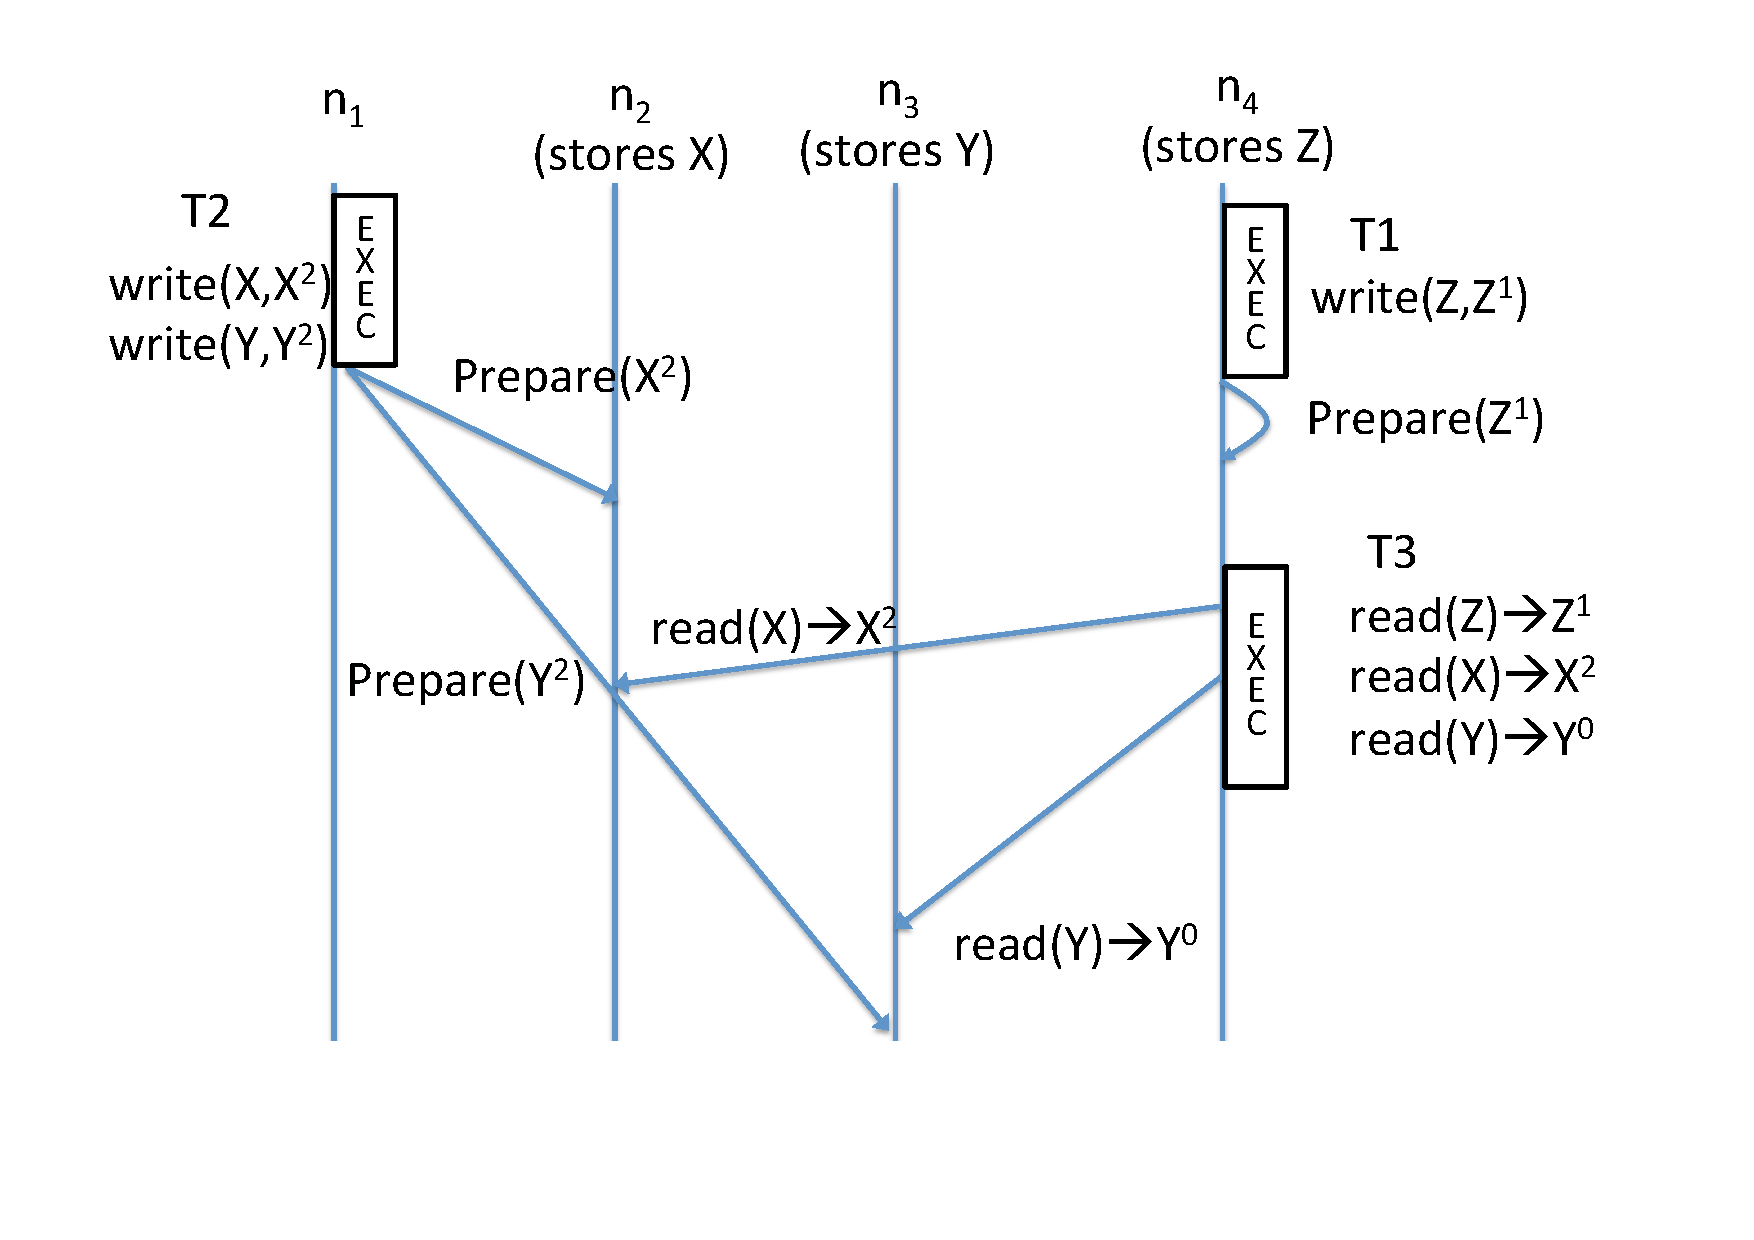
\includegraphics[scale = 0.24]{figures/example.pdf}
\caption{\footnotesize Example concurrency anomaly that may arise when adopting weak-consistency models that do not abide by the SPSI criterion.}
\label{fig:example}
\end{figure}

The system proposed in this paper, which we called \specula (Speculative Transactional Replication), provides developers with the flexibility of choosing between two different consistency semantics for the transactions that compose their applications: a strong consistency semantics, i.e., the familiar Snapshot Isolation~\cite{berenson1995critique}, and a weakly consistent one, which we termed Speculative Snapshot Isolation (SPSI). The idea of unifying different consistency models within the same programming model is not new: two notable examples are the red-blue consistency model recently proposed in Gemini~\cite{li2012making} and the support in SQL for specifying different isolation levels on a per transaction basis~\cite{sqk}.  The main innovative aspect of \specula lies in its novel transactional replication protocol, which provides unique advantages with respect to state of the art systems that provide either strong or weak consistency semantics (or both).

~\\
\noindent {\bf Strong consistency semantics:} 
\iffalse
The protocol employed by \specula to ensure strong consistency shares several key design choices with state-of-the-art data stores~\cite{spanner,clock-si,PelusoScore}, which contribute to its efficiency and scalability. These include:  multi-versioning, which maximizes efficiency in read-dominated workloads~\cite{bernstein-book},  distributed clocks, which are used to establish the transaction serialization order in a fully decentralized fashion,~\cite{spanner} as well as support for partial replication, a  feature that is generally regarded as fundamental to achieve high scalability~\cite{kemmeAndRicardo,PelusoGMU}. 
\fi
\specula supports transactions with strong consistency semantics, i.e. Snapshot Isolation, which provides programmers the familiar ACID properties. However, comparing with conventional transactional protocols, \specula takes a radically different approach regarding the management of transactional conflicts involving pre-committed data. Existing strong-consistent protocols take a conservative approach, which prevents any transaction T from ever observing the data item versions pre-committed by a different transaction T' --- either by blocking T till T' commits, or by letting T observe the pre-image of the execution of T'. This choice is arguably motivated by the fact that allowing transactions to observe pre-committed data item versions exposes them to the risk of cascading aborts~\cite{xxx}, a property that is ``historically'' deemed as crucial to maximize the efficiency of a transactional system~\cite{textbooks-on-db}. \specula departs from these conventional designs, and embraces a speculative approach that spares transactions that incur a conflict on pre-committed data from having to wait for the finalization of the commit phase of the lock-holding transaction. Conversely, \specula's distributed concurrency control mechanism takes an optimistic approach, i.e., it speculates on the eventual success (i.e., commit) of pre-committed transactions and allows the data versions pre-committed by a transaction T to be read by concurrent transactions, that are hence speculatively serialized after T. As we will show via an extensive experimental study, \specula's design choice of allowing speculative read can lead to increase throughput by up to XX$\times$ and reduce latency by up to YY$\times$. A striking, and more general, result stemming from our work is that, in strongly consistent geo-replicated data stores, the advantages stemming from accepting the risk of cascading aborts largely outweighs its drawbacks, leading to remarkable gains in terms of both throughput and latency.

~\\
\noindent {\bf Weak consistency semantics:} Analogously to the well-known eventual consistency model~\cite{brewer2012cap}, the weak consistency model supported by \specula, i.e., SPSI, allows application developers to \textit{speculative commit} transactions, i.e., to externalize to its users (e.g., human operators) the results of a transaction while this is still undergoing its final commit/certification phase. As such, when programmers choose to exploit the speculative commit capabilities of \specula, they also need to develop compensation logic for coping with the case in which a speculatively committed transaction has to be eventually aborted.

What distinguishes SPSI from existing weak consistency models is that it provides clear and stringent guarantees on the atomicity and isolation of the snapshots observed and produced during transactions' execution. Figure~\ref{fig:example} illustrates one of possible concurrency anomalies that can arise in a transactional system that adopts weak consistency, by exposing the data item versions produced by speculatively committed transactions: transaction T3 observes the version of data item X precommitted by a concurrent transaction, T2, on node n$_1$. However, when it comes to reading Y, which was also updated by T2, T3 misses the version created by T2 on node n$_3$ (as T2's updates are still being propagated to node \textit{n$_2$}). Such concurrency anomalies are prevented by the SPSI specification, which, in a nutshell, guarantees that the snapshots that can be observed/speculatively committed by a transaction T originated at a node \textit{n}
%
% observable by \textit{any} transaction (independently of whether they ) and those that are produced by a speculatively committed transaction T 
% 
 are equivalent to the ones that would have been observed/committed by T, had it been executed by a non-speculative SI data store along with a subset of all the transactions existing in the system, which excludes any concurrent, speculatively committed transaction originated at a node $n'\neq n$.
% 
% 
%  
% 
%  processed a subset of the entire set of transactions existing in the system that does include specu which comprises all the transactions that, by the time T started,  i) had either finalized their commit phase or ii) were activated on the same node that originated T and had speculatively committed.
 On the one hand,  SPSI  spares programmers from complex concurrency bugs, by ensuring that  transactions always execute on snapshots that are atomic and isolated, although not capturing the effects of concurrent, speculatively committed remote transactions. On the other hand, by demanding that the snapshots over which transactions execute reflect \textit{only} the effects of locally activated concurrent transactions, SPSI's specification allows for efficient implementations that can decide whether it is safe to speculatively commit a transaction solely on the basis of local information.

%, as illustrated in the example execution in Figure~\ref{example}, and ii) it makes transactions subject to cascading-aborts~\cite{xxx}, a property that is ``historically'' deemed as important for the efficiency of a transactional system. \specula rules out the former risk, thanks to an innovative, fully distributed, multi-versioned concurrency control scheme
%
%such data item to be ever observed, by blocking the  transaction requesting access to the data item or
%
%, though, departs from one of the key a
%
%
%
%Still, the latency and performance cost for guaranteeing consistency results seems indispensable. For example, logically a banking system should always be execute with strong consistency, as monetary loss caused by inconsistent operations seems unacceptable \cite{li2012making}. Interestingly, this is not always the case for systems used in daily life. Brew et al. described the design of a practical automated teller machine (ATM): when an ATM experiences network partition, it indeed takes the risk of overdrafting accounts to allows withdrawal unilaterally. In fact, ATM's ability to dispense money outweighs the trouble caused by account overdraft. Accidental overdraft will be handled by a well-defined external compensation logic \cite{brewer2012cap}.
%
%The design of the described ATM comes from a profound insight: practical applications may not always need 100\% consistency guarantee; instead, as long as the latency and availability benefit pay off the cost of compensating occasional mistakes, they may take risks, i.e. speculate on the result of operations, instead of pessimistically waiting out uncertainty \cite{helland2009building, brewer2012cap, bailis2013eventual}. In light of this, this paper presents {\specula}, a distributed transactional key-value store that exploits speculation to circumvent the inherent large latency and low throughput of strongly-consistent transactions. The main goal of \specula is to endow application developers the flexibility to speculate transactions for latency and throughput, while keeping programming complexity in check.
%
%\specula consists of a programming interface and a speculative transaction protocols. The programming interface allows programmers to exert control over speculative transaction: programmers develop application with strong consistency by default, but also have the choice to specify transactions to execute in a speculative fashion, without affecting other transactions. \specula 's speculative transactional protocol enables efficient transaction processing and ensures meaningful semantics, namely SPeculative Snapshot Isolation (SPSI), to programmers. Previous research works have exploited different aspects of speculation execution \cite{kraska2009consistency, pang2014planet}: Consistency Rationing \cite{kraska2009consistency} proposes cost models to measure the best tradeoff of consistency and cost; PLANET \cite{kraska2009consistency} proposes a speculative programming interface and calculates the commit probability of transactions. However, to the best of knowledge, we are the first to propose a speculative transactional protocol for modern large-scale, fully decentralized datastore.
% &  111 &  Haha &  Stupdi &  Noway & ahaha &   \\ \hline

Overall, this paper makes three main contributions:
~\\
\noindent {\em 1.} We propose SPeculative Snapshot Isolation (SPSI), a consistency criterion ad hoc designed for speculative transactional systems. SPSI extends the notion of Snapshot Isolation in an intuitive way, in order to provide meaningful consistency guarantees to transactions observing speculatively committed data (\S \ref{sec:overview}, \ref{sec:protocol}).
~\\
\noindent {\em 2.} We present the design of \specula, a  geo-replicated data store that exploits a novel, fully-decentralized, highly scalable protocol that efficiently supports speculatively transaction execution in presence of partially-replicated data  (\S \ref{sec:protocol}).
~\\
\noindent {\em 3.} We conduct an extensive experimental evaluation (\S \ref{sec:evaluation}),  encompassing both complex/realistic benchmarks (TPC-C and Rubis) and synthetic micro-benchmarks that allow us to exercise a wide range of diverse workloads. The results of our study highlight that:
\begin{itemize}
\item \specula's innovative speculative concurrency control ensures strong consistency (SI) with  average  gains of XX\% in throughput and YY\% in latency with respect to state of the art systems, with peak gains that extend up XX$\times$ for throughput and YY$\times$ for latency. 
\item Applications that adopt \specula's weak consistency semantics (SPSI) can reduce the user-perceived latency, on average  (i.e., considering both scenarios of successful and unsuccessful speculation), by an additional XX\% factor. Further, \specula's weak consistency semantics   allow for enhancing the throughput achievable by \specula by up to XX$\times$ in machine-to-machine applications in which the rate of submission of new transactions is solely throttled by the speed at which the system can process previously submitted transactions.
\end{itemize}

The remainder of this paper is structured as follows. {\bf TODO}


\section{Related Work}
The problem of designing efficient mechanisms to ensure strong consistency semantics in geo-replicated data stores has garnered considerable interest in both industry and academy. Two notable examples are Spanner \cite{spanner} and SDUR \cite{scatter}, which  provide strongly consistent transactions via the use of Two-phase commit and Paxos. As already mentioned, \specula builds on state of the art partially replicated geo-distributed data stores, with which it shares several design decisions that contribute to its efficiency and scalability. However, it extends them with innovative speculative concurrency control techniques.

The literature has explored a number of alternative approaches to mitigate, or even possibly avoid, the costs of inter-data-center synchronization in geo-replicated data stores. A first class of approaches consists of protocols  optimized on the basis of the assumption that data is fully replicated across different data-centers, i.e., each data-center maintains a full image of the system's data. To this end, Replicated Commit~\cite{mahmoud2013low} runs Two-Phase Commit multiple times
in different datacenters and then uses Paxos to reach consensus as to whether the transaction should commit; MDCC~\cite{kraska2013mdcc} uses Generalized Paxos \cite{lamport2005generalized} to commit transaction, which takes only a single WAN round-trip in normal case. Unlike these works, \specula supports a more generic and scalable data-model, in which data can be partially replicated across a subset of the available data-centers.

 
 Other recent approaches~\cite{zhang2013transaction,SwiftCloud,Walter} have aimed to reduce the cost of enforcing strong consistency, e.g., by identifying (possibly in a semi-automatic way) and exploiting the presence of commutative operations that can be executed without endangering consistency (as they are guaranteed  to never conflict). Bumper~\cite{Diegues2013SRDS}  focuses on the problem of contention hot-spots, allowing to postpone the execution of conflict-prone operations issued within a transaction till their commit phase --- where they are executed after having acquired all the locks they require, and hence without risking to incur aborts. These approaches are orthogonal to \specula and  these mechanisms  could be combined with the speculative techniques  at the heart of \specula's replication protocol to further enhance its performance.
 
Reducing the cost of inter-replica synchronization by relaxing the consistency semantics  provided to applications is another well-explored idea in the literature. Gemini~\cite{li2012making}, for instance, requires programmers to analyze applications and identify (possibly with the aid of static analysis tools~\cite{atc-rodrigo}) which subset of application's operations commute and can safely take advantage of weak consistency semantics.  Unlike \specula, Gemini, assumes a fully replicated data model and, as such, it does not address the issue of how to achieve isolation in presence of operations/transactions that require accessing  multiple data items scattered across different machines (see Figures~\ref{fig:ex1} and~\ref{fig:ex2}). 

Kraska et. al. allows programmers to specify which data shards demand strong consistency (serializability)  and which ones can  tolerate weak semantics (session guarantees), albeit possibly at some cost. This information is then exploited to dynamically adapt the consistency provided to transactions and reach an optimal balance between consistency and latency \cite{kraska2009consistency}. This approach only guarantees the weakest consistency semantics to transactions that access both weakly and strongly consistent data shards. Conversely, \specula ensures strong consistency semantics, as specified by the SPSI criterion, in 

Xie et. al.~\cite{xie2014salt} propose Salt Isolation, which allows classic ACID transactions to co-exist with BASE transactions, i.e., weakly consistent transactions that can externalize their intermediate state to minimize lock duration. Analogously to SPSI, Salt ensures that strong consistent transactions are not affected by the execution of weak consistent ones. However,  \specula ensures that \textit{any} transaction always observes and produces atomic and isolated snapshots, although potentially not reflecting the execution of concurrent transactions originated at different nodes. As discussed in \S \ref{sec:introduction}, this design choice spares programmers from the complexity of reasoning on subtle concurrency bugs that may lead applications running in non-sand-boxed environments  to exhibit arbitrary behaviours~\cite{opacity, virtualWorldConsistency}: this is the case, for instance, of applications that do not access data via well-defined query languages, like SQL, but rather by embedding transactions into arbitrary code written in a general purpose programming language, like Java~\cite{javaPersistenceAPI}. In the former case, inconsistencies lead to stale data being returned, but will not cause the data-store to crash. In the latter case, instead, inconsistencies can lead applications to crash because of unexpected exceptions or to enter infinite loops~\cite{transactionsAreBackButTheyAreNotTheSame}. 


The idea of exposing, in a speculative fashion, the post-image produced by locally, but not yet globally, certified transactions is not new in the literature. The programming model exposed by PLANET \cite{pang2014planet}, analogously to \specula's,  aims to reduce the user-perceived latency by letting programmers expose the results of speculatively committed transactions. Unlike \specula, though, PLANET relies on a conventional/non-speculative data replication scheme that  never exposes pre-committed data to transactions. As such, PLANET can only benefit user-perceived latency, but fails to reduce the transaction's blocking time and, hence, to enhance throughput and reduce the time it takes to finalize the processing of a transaction. 
The idea of letting transactions ``optimistically'' borrow, in a controlled manner, the updated data of transactions currently in their commit phase has already been investigated in the past. Several works, e.g., SPECULA \cite{peluso2012specula} and Aggro \cite{palmieri2010aggro}, have applied this idea in contexts that are radically different from the ones considered in this paper, i.e.,  small scale clusters in which  data is fully replicated via total-order based coordination primitives. Conversely, \specula is designed for partially replicated data-stores distributed over geographical scale that ensure consistency via Two-phase commit.  SCC-kS~\cite{bestavros1996value}, PROMPT~\cite{PROMPT} and SL~\cite{Reddy} target a relatively closer system model, i.e., distributed databases, but do not support data replication and multi-version concurrency control. These are two mechanisms that are regarded as essential in modern, large scale online services~\cite{spanner,megastore,score}. Further, some of these proposals ~\cite{bestavros1996value, Romano-2014} rely on complex graph-based concurrency control techniques, whose efficiency has also been evaluated via simulation and that are likely to suffer from large overheads in realistic settings. Finally, unlike \specula, PROMPT, SL and SCC-kS may expose non-atomic/isolated snapshots during transaction's execution.
\section{System  and data  model}
\label{sec:overview}

Our target system model encompasses a set of geo-distributed data centers, each hosting a (typically large) set of servers, or nodes. 
In the following, we shall assume a key-value data model. This is done for simplicity and since  our current implementation of \specula runs on a key-value store. However, the protocol we present  is agnostic to the underlying data model (e.g., relational or object-oriented). 

The whole dataset is partitioned across multiple replicated shards, or partitions.
Each data partition is responsible for a key range and it maintains multiple timestamped versions for each key.  Synchronous master-slave replication is employed to enforce fault tolerance and transparent failover, as used in \cite{spanner, baker2011megastore}. A partition has a master replica and several slave replicas, and, at commit time, update transactions contact the masters of the partitions they accessed. These verify whether transactions can be correctly serialized  and propagate their updates, along with any metadata (e.g., locks held by the transaction) required for their recovery, to its replicas.
This scheme allows for transparent fail-over, in case of failure of master replicas. Further, it allows reads to be served by any replica, which allows client to freely select the one that is geographically closer.


Partitions may be scattered across the nodes in the system using arbitrary data placement policies. A server can host multiple data partitions, either master replicas or slave replicas. A data partition can be replicated within a datacenter and across datacenters. Also, no server or datacenter is required to host all partitions. 

In absence of failures, the distributed concurrency protocol presented in \S \ref{sec:protocol} does not rely on any synchrony assumption, i.e., it is designed operate in a pure asynchronous system. It only requires that  servers are equipped with loosely synchronized, conventional hardware clocks, which we only assume to monotonically move forward. Additional synchrony assumptions, though, are required,  in presence of failures~\cite{fischer1985impossibility}, to ensure the correctness of the synchronous master-slave replication scheme embedded in \specula's protocol. Our current prototype employs a classic primary-backup approach, which assumes perfect failure detection capabilities~\cite{chandra1996unreliable}. However, it would be straightfoward to replace the current replication scheme to use, e.g., Paxos~\cite{lamport2005generalized}, which  allow for weaker synchrony assumptions~\cite{dwork1988consensus}.


%Analogously to other recent geo-distributed data stores~\cite{spanner, clocksi, terry2013consistency}, \specula supports flexible data placement policies. A server can host multiple data partitions, either master replicas or slave replicas. A data partition can be replicated within a datacenter and across datacenters, and no server or datacenter is required to host all partitions. 



\section{Programming Model}
\label{sec:programming_model}


%ACID transactions provide a powerful programming abstraction by ensuring Atomicity, Consistency, Isolation and Durability. To enforce these properties, ACID transactions specify a set of rigorous execution rules, which often require synchronization between geo-dispersed data replicas. In state of the art data stores, like Google's Spanner~\cite{spanner}, committing a transaction entails the execution of a two phase commit protocol among the master of different partitions along with a consensus instance among the replicas of each partition~\cite{cockroach,spanner,schiper2010p}. These protocols introduce in the critical path of the commit phase the latency of several inter-datacenters communication steps, which is detrimental to user experience \cite{schurman2009user}.
%
%An intuitive way to mask this large inter-datacenters latency is to make an optimistic guess about the result of a transaction, instead of waiting out the uncertainty. The consequence is that, rather than always getting correct and irrevocable results, clients get predicted results that may occasionally go wrong. As we have discussed in \S \ref{sec:introduction}, although replying users with a probably correct answer, instead of a definitive one, seems unacceptable in an idealistic business model, it is indeed commonly used in practice \cite{helland2009building, brewer2012cap}, to tame large latency and low availability: an ATM allows clients to withdraw money even in the presence of network partition, and charges users overdraft fees if necessary; flight companies usually oversell tickets to ensure high occupancy rate, to achieve higher revenue while risking compensating passengers that could not get booked seats.
%
%Allowing speculative commit raises a relevant question: if clients try to read pending updates of speculatively-committed transactions, how should the system react? A straw-man proposal is to ignore these speculative versions (by returning the last committed version or blocking clients until these versions are committed or aborted), therefore transactions still execute in a strongly-consistent fashion and no extra complexity is introduced (as exploited by \cite{pang2014planet}). Albeit neat, this approach has potential problems: returning older versions gives clients weird semantics, while blocking until speculative updated are finalized can introduce large latency especially when the system has hotspots. To avoid these problems, \specula allows speculatively-committed transactions' updates to be visible to others transactions. In further sections, we shall more precisely define the consistency semantics (\S \ref{subsec:ssi}) as well as how the protocol design.
%
%\iffalse
%The prevalence of geo-replication has fueled the Eventual Consistency (BASE transactions) v.s. Strong Consistency (ACID transactions) argument. While achieving high availability and low latency by avoiding inter-datacenter latency, eventual consistency only guarantees that ``...changes made to one copy eventually migrate to all", according to one of its earliest definitions \cite{kawell1988replicated}. Programmers have to explicitly code ad-hoc logic to deal with concurrency anomalies and ensure consistency requirements. On the other hand, strong consistency provides a powerful programming abstraction via enforcing a set of rigorous execution rules, which often requires synchronization between geo-dispersed data replicas. In state of the art data stores, like Google's Spanner~\cite{spanner}, committing a transaction entails the execution of a two phase commit protocol among the master of different partitions along with a consensus instance among the replicas of each partition~\cite{cockroach,spanner,schiper2010p}. These protocols introduce in the critical path of the commit phase the latency of several inter-datacenters communication steps. Such a latency can not only have a detrimental impact on user experience in human-facing interactions~\cite{schurman2009user}, but also lead to lock convoying effects that can severely hinder concurrency and throughput.
%\fi

This section discusses how to extend the conventional programming model exposed by (non-speculative) transactional systems to encompass the two speculative techniques that we investigate in this work, namely speculative reads and speculative commits.

The integration of a speculative transaction processing technique in the programming model raises different issues depending on whether recovery from mispeculation can be automatically achieved by the transactional system, or whether it entails the development of application-dependent compensation logic. Based on this rationale, we identify two classes of speculative techniques, which we call, respectively, \textit{internal} and \textit{external} speculation.

Speculative reads (as well as, e.g., optimistic concurrency control~\cite{berenson1995critique}) belong to class of internal speculation techniques, as the effects of mispeculation remain hidden from the clients until the transaction is committed, either in a speculative or non-speculative fashion. The system can hence recover from a mispeculation by simply aborting and restarting the corresponding transaction. Speculative commits, conversely, belong to the class of external speculation techniques, as the logic for coping with mispeculation scenarios in which a transaction aborts after having externalized its results  (via a speculative commit) is inherently application-dependent~\cite{bailis2013eventual}. As such, depending on a number of application-dependant factors, the cost and complexity associated with the development and execution of compensation logic for speculatively committed transactions may be unacceptably large.

The programming model we propose in this work builds on these considerations by empowering  developers to circumscribe the scenarios in which speculative commits should be used and to exploit application-dependant information to maximize the chance of successful speculation.

This result is achieved by extending the conventional API used to start a transaction, which we encapsulate in the \textit{beginTx} primitive, to accept as input four parameters:\\
\noindent $\bullet$~\textsc{canSpecCommit}, a callback that is activated when the transaction execution is completed, i.e., the transactions issues a commit request. The callback must return a boolean value that determines whether the transaction should be allowed to undergo a speculative commit, or not. This allow programmers to exert fine-grained control on which transaction instances should be speculatively committed.  This callback executes within the same context of its corresponding transaction. This guarantees that any data-item access issued from within this callback is executed on the same data snapshot observed by its corresponding transaction. \\
\noindent $\bullet$~three additional callbacks, i.e., \textsc{specCommitHandler}, \textsc{finalCommitHandler}, and \textsc{finalAbortHandler},  which allow  programmers to specify the application-dependent logic that should be executed upon a speculative commit, a final commit or if a transaction is aborted after having been speculatively committed, respectively. Like \textsc{canSpecCommit}, the \textsc{specCommitHandler} handlers executes in the same  scope of the transaction it is associated with. Conversely, final commit and final abort handlers callbacks do not execute in the same context of the transaction they are associated to. This is unavoidable since these handlers are executed only after the transaction's outcome has been already determined. 




 

The callbacks specified in \textit{beginTx} can obtain additional information related to the transaction execution via  an in-memory map called \textsc{TxInfo}. To this end, transactions can programatically store in \textsc{TxInfo}  any information that could be relevant for its callbacks (e.g., the transaction's input parameters). \textsc{TxInfo} can also used by the speculative transactional system to make available statistical information on the effectiveness of speculation for a specific type of transaction (e.g., how often speculative commits are followed by a final commit event).


No additional changes to the conventional APIs of a non-speculative transactional system are required, which contributes to minimize the complexity faced by developers who wish to embrace the proposed speculative programming paradigm to enhance the performance of their applications. 




Listing 1 illustrates the use of the proposed API through an example code of a simplified online shopping transaction. In the considered example, the checkRisk callback allows a transaction to be speculatively committed only if it is buying an inexpensive item and has experienced a low abort rate over a recent time-window. The former information is programmaticaly stored  in the \textsc{TxInfo} map during transaction's execution, whereas the latter is updated by the speculative data store in a fully transparent way for application developers. The example code presents a simple approach that aims to reduce the frequency with which mispeculation need to be actually exposed to the final-users of the system: since the semantics of buying an item does not change during different runs, the system can just retry a few times the buy item transaction if it gets aborted after speculation


\begin{lstlisting}[caption=Example use case of the proposed programming model.]   
checkRisk() { 
    return TxInfo.get("ItemPrice") < 100 &&
                    TxInfo.get("CommitProb") > 0.9
}

scHandler() {
    // Display "Your order has been placed."
}

fcHandler() {
    // Send an email to the user notifying success order
}

faHandler() {
    // Retry three times, if still fails then,
    // Apologize with the user via email.
}

buyItemTx(ItemInfo){
    Tx = beginTx(
                checkRisk(),//Allow speculative commit?
                scHandler(),//Speculative commit callback
                fcHandler(),//Final commit callback
                faHandler());//Final abort callback
    Item = tx.read(ItemInfo);
    Item.quantity -= 1;
    Tx.write(ItemInfo, Item);
    TxInfo.put("ItemPrice", Item.price);
    Tx.commit();
}
\end{lstlisting}
%{\bf Enabling speculative commits and/or reads.} \specula extends the transaction begin API with two optional boolean parameters, namely \textit{specCommit} and \textit{specRead} (which default to true if they are left unspecified). The former allows programmers to define whether a transaction should be speculatively committed: as in the example, programmers specify a \textit{checkRisk} function to decide whether to perform speculative commit. We shall define more rigorously the consistency guarantees ensured by \specula for a speculatively committed transaction in the next section. 
%\iffalse
%Yet, in a nutshell, a speculatively committed transaction is guaranteed to have executed respecting the SI semantics for a history comprising all final committed transactions and locally originated speculatively committed transactions.
%\fi
%
%
%As illustrated in the code example, the use of these two flags empowers application (or middleware) programmers to craft logic aimed to maximize the chance of successful speculation, as well as to circumscribe the scenarios in which speculation should be used. For instance, in the considered example, a transaction can be allowed to be speculatively committed only if it is buying an inexpensive item and if it has experienced a low abort rate over a recent time-window, and is allowed to read speculatively committed data versions. Yet, the two flags can be used independently. For instance, a developer may decide to allow a transaction $T$ to observe speculatively committed data versions even though $T$ is not allowed to speculative commit. This may enhance the chances of having $T$ commit, by ensuring that $T$ can read the versions generated by concurrent speculatively committed transactions, while avoiding to ever expose speculative state to the client that issued $T$.

%It should be noted that enabling the possibility of observing speculatively committed data version raises subtle issues.  Snapshot Isolation (SI) has not been defined with speculation in mind. In particular, it does not specify which data snapshots should be observable in histories encompassing speculatively committed transactions. We cope with this issue in the following Section, in which we shall introduce a generalization of SI, called SPeculative Snapshot Isolation (SPSI), that will serve as target consistency criterion for \specula.


%{\bf Reacting to Speculative Commit and Final Commit/Abort Events.} Upon beginning a new transaction, programmers have to specify three callback functions: \textit{onSpeculativeCommit()}, \textit{onFinalAbort()} and \textit{onFinalCommit()}.

%As its name suggests, onSpeculativeCommit() allows programmers to define which code should be executed if a transaction is speculatively committed (i.e., it passes local certification). Furthermore, the other two callbacks (\textit{onFinalAbort()} and \textit{onFinalCommit()} ) specify the actions to take when a transaction is eventually committed or aborted after speculative commit, respectively. The example code presents a simple way to avoid notifying users too often about speculative abort: since the semantics of buying an items does not change during different runs, the system can just retry the buy item transaction if it gets aborted after speculation.

\section{Speculative Snapshot Isolation}
\label{subsec:ssi}
As mentioned above, SPSI has been designed to generalize the well-known SI criterion and define, in a rigorous yet intuitive way, the consistency semantics guaranteed to user-level applications when using speculative transaction processing techniques.

Before presenting the SPSI specifications, we first recall the definition of SI~\cite{weikum2001transactional}:

\begin{itemize}
\item \textsc{SI Property 1.} (\textit{Snapshot Read}) All operations read the most
recent committed version as of the time when the transaction began.
\item \textsc{SI Property 2.} (\textit{No Write-Write Conflicts}) The write sets of
each pair of committed concurrent transactions must be disjoint.
\end{itemize}

The design process that led us to the definition of SPSI has been driven by three main goals/requirements:
\begin{itemize}
\item simplify application's development by preventing subtle concurrency anomalies (like the atomicity and isolation violations illustrated in Figures~\ref{fig:ex1} and~\ref{fig:ex2}) that may arise in systems that allow transactions to speculatively observe pre-committed data or externalize speculatively committed data;
\item preserving the intuitiveness and simplicity of the original SI specification;
\item enabling highly scalable and efficient implementations, in which transactions can be speculatively committed based only on local certification activities.
\end{itemize}


Guided by these three objectives, we specify SPSI via the following properties:
\begin{itemize}
\item \textsc{SPSI Property 1.} (\textit{Speculative Snapshot Read}) A transaction $T$ originated at a node $S$ must observe the most recent data item versions created by the transactions that i) have final committed by the time $T$ started (independently of the site where these transactions originated), or ii) have speculatively committed by the time T started and were also originated at node $S$.
\item \textsc{SPSI Property 2.} (\textit{No Write-Write Conflicts among Final Committed Transactions}) The write sets of
each pair of finally committed concurrent transactions must be disjoint.
\item \textsc{SPSI Property 3.} (\textit{No Write-Write Conflicts among Speculatively Committed and Committed Transactions}) The write sets of a speculatively committed transactions originated at a node $n$ must not intersect with the write-set of any concurrent transaction that i) has been final committed, or ii) has been speculatively committed and originated at node $n$.
\item \textsc{SPSI Property 4.} (\textit{No Dependencies from Aborted Transactions}) A transaction can only be final committed if it does not depend on a speculatively committed or aborted transaction.
\end{itemize}

SPSI Property 1 extends the notion of snapshot, at the basis of the SI definition, to include among the set of  transactions visible to a transaction $T$ originated on a node S at time $t$ all the transactions that have also originated on $S$ and that were speculatively committed by time $T$. Notice that this guarantee applies to all transactions, including those that have to be eventually aborted due to conflicts with either local or remote transactions. This property provides the illusion that a transaction $T$ executes on an immutable snapshot, which reflects the execution of all the transactions speculatively committed before $T$'s activation, and originated on the same local node. 

SPSI Property 2 coincides with SI's property 2, ensuring the same semantics regarding the absence of write-write conflicts among concurrent final committed transactions. SPSI Property 3 expresses analogous guarantees for speculatively committed transactions, although with a relevant difference: such guarantees are restricted only to pairs of transactions that are originated at the same node. It is worth highlighting that the choice of restricting, in SPSI Properties 1 and 3, the guarantees regarding speculative committed versions only to transactions originated at the same site is fundamental to allow implementing efficient schemes that can decide whether to speculative commit a transaction based solely on local knowledge (i.e., avoiding expensive remote certification phases).

Finally, SPSI Property 4 ensures that a transaction can be final committed only if it does not have any \textit{dependence} on transactions that are not, in their turn, final committed.
We distinguish two types of dependencies: \textit{flow dependencies} and \textit{data dependencies}. Flow dependencies  between two transactions T and T' are developed whenever a given client activates T' after having speculatively committed T and are only removed when the final outcome (i.e., commit/abort) for T is determined. This allows to capture  causal dependencies that arise when a client activates a new transactions on the basis of the results produced by any speculatively committed transaction that was previously activated by the same user. For instance, a flow dependence is established if a user decides to activate a hotel booking reservation after having observed the speculative commit of a fight reservation: in case the flight reservation transaction is eventually rolled back, SPSI forces to abort also the hotel booking transaction. We say that transaction T has a data dependence on transaction T' if T speculatively reads data pre-committed by T'. 
Overall, SPSI Property 4  guarantees that whenever a transaction final commits, it can not causally depend on any  transaction whose outcome is not determined yet, and may hence eventually abort.

Overall, SPSI Properties 1, 3 and 4 greatly restrict the spectrum of anomalies that can be experienced by speculatively committed transactions, by limiting them to conflicts developed with concurrent transactions originated at remote sites. More formally, those properties ensure that applications that expose/observe speculative states always produce/execute on snapshots  that are correct if one applies the SI criterion to the transaction history comprising the transactions which were known to the node in which such applications executed at the time in which they started executing a transaction. 


\section{The \specula protocol}
\label{sec:protocol}
This section presents the \specula protocol. First (\S \ref{subsec:baseline}), we give an overview the protocol, introducing the key techniques that differentiate it from conventional transactional protocols. Next (\S \ref{subsec:execution}), we describe the protocol in detail. Finally, we discuss about the fault tolerance of \specula and how to control the aggressiveness of speculation.

\iffalse
\subsection{Transaction execution}
Figure \ref{fig:txn_state} presents the execution state diagram of a speculative transaction.

\begin{figure}[t]
\centering
\hspace{-6mm}
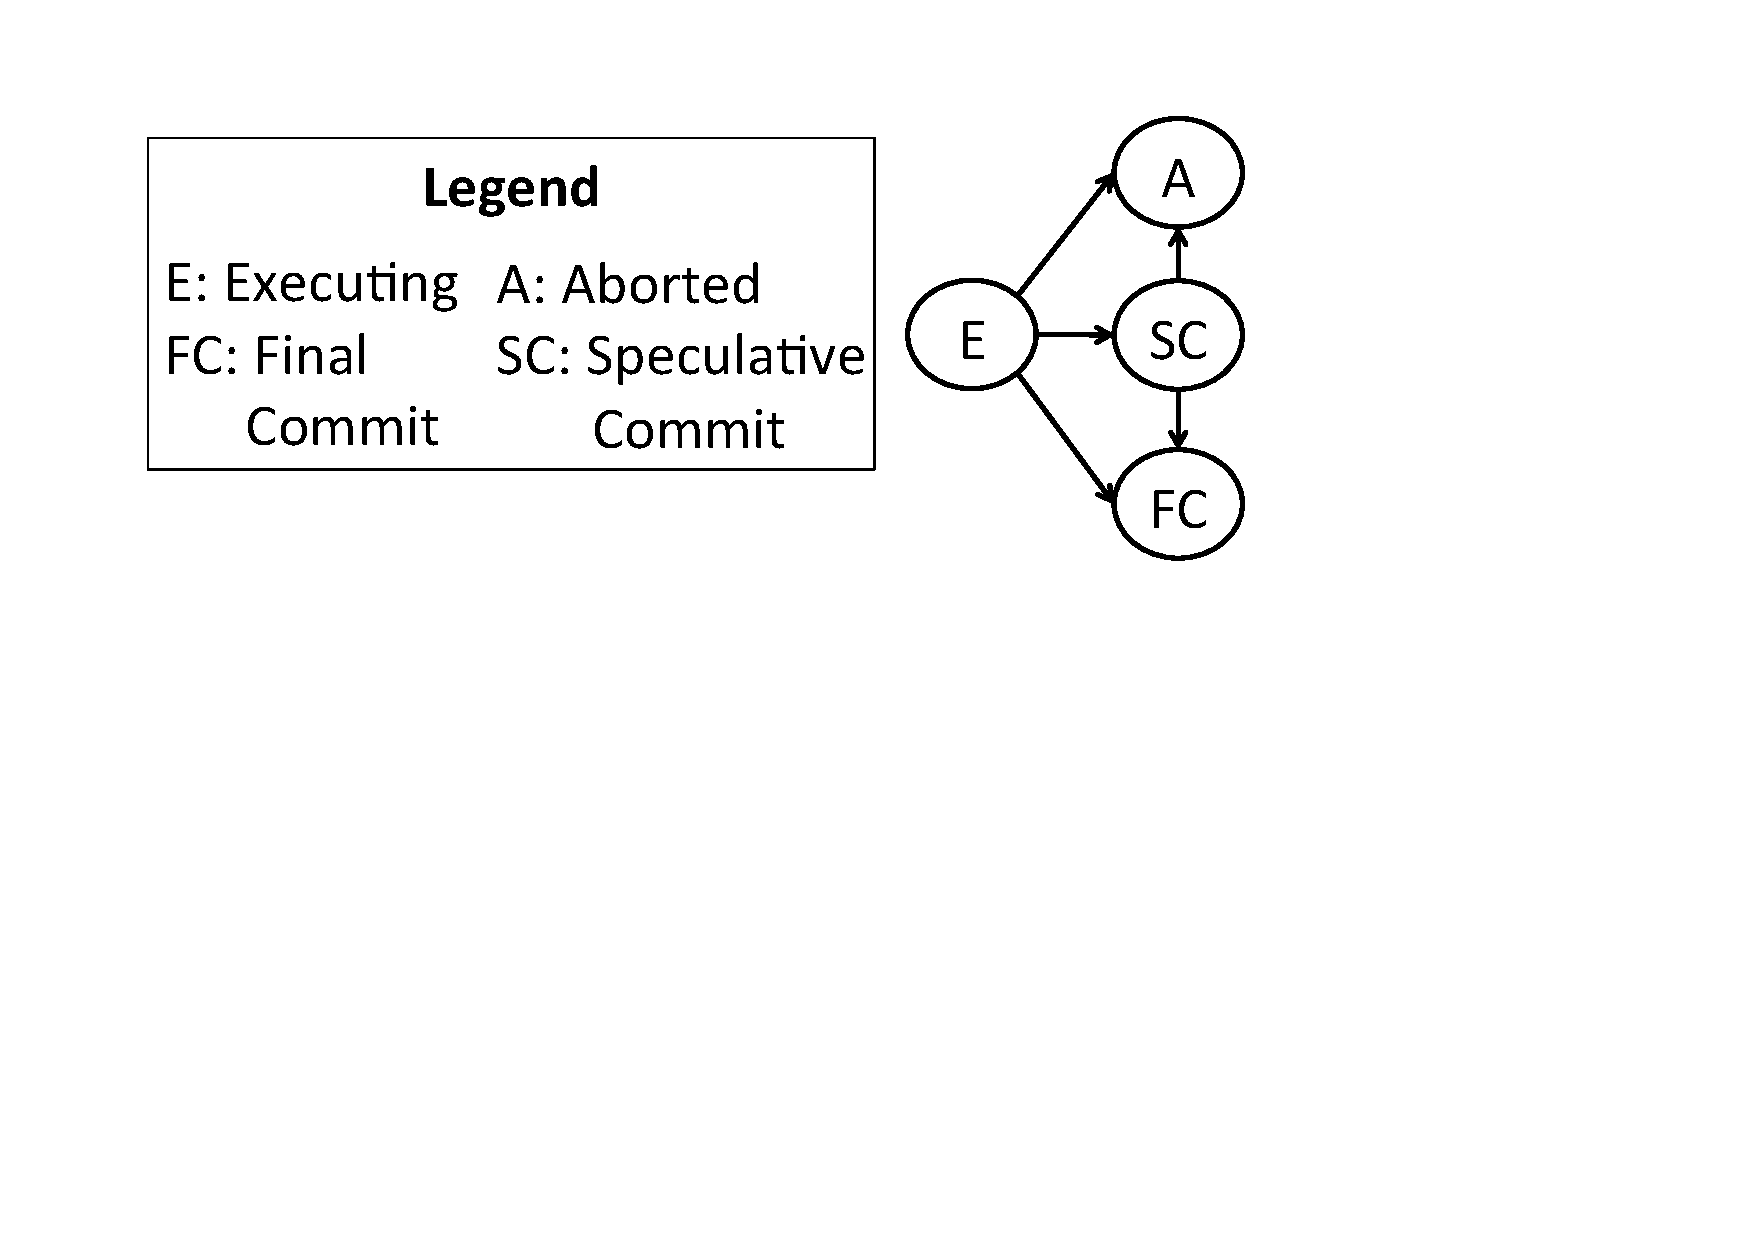
\includegraphics[scale = 0.3]{figures/state-machine.pdf}
\caption{Diagram illustrating the possible state transitions of a transaction in \specula.}
\label{fig:txn_state}
\end{figure}
\fi

\begin{figure}[t]
\centering
\begin{subfigure}[t!]{0.95\linewidth}
\def\svgwidth{0.95\columnwidth}
\centering 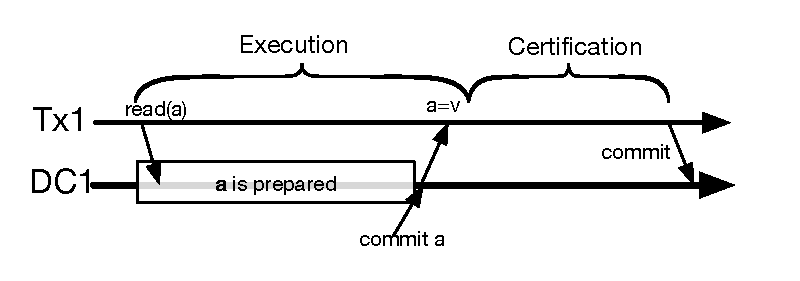
\includegraphics[scale = 0.65]{figures/NoSpeculativeRead}
\vspace{-8mm}
\caption{\footnotesize Not allowing reading pre-commit values.}
\label{fig:remote:a}
\end{subfigure}

\begin{subfigure}[t!]{0.95\linewidth}
\vspace{1mm}
\def\svgwidth{0.95\columnwidth}
\centering 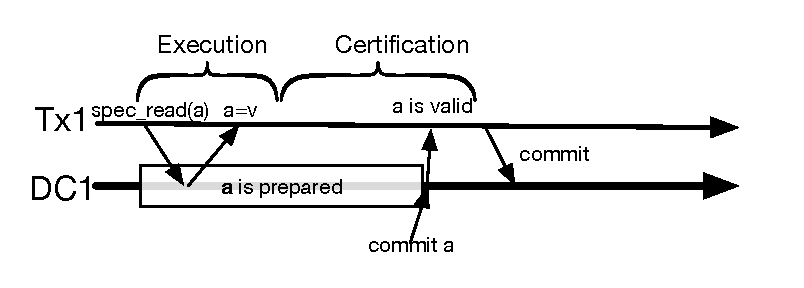
\includegraphics[scale = 0.65]{figures/YesSpeculativeRead}%Remotereadremoteread
\vspace{-5mm}
\caption{\footnotesize Speculatively reading pre-commit values.}
\label{fig:remote:b}
\end{subfigure}
\caption{The performance benefit of speculative read.}
\label{fig:specularead}
\end{figure}


\subsection{Protocol overview}
\label{sub:sc}
At its core, \specula is based on transactional protocols that employ optimistic concurrency control \cite{clocksi, mdcc}: a transaction typically has a short execution phase where it performs multiple read and write operations, then it tries to commit by certifying its write-set, during which pre-commit locks are maintained on data items being certified. Unlike these conventional protocols, \specula optimistically exposes these pre-commit versions to other transactions, which can reduce transaction's waiting time and increase throughput (\ref{fig:specularead}). Although a naive modification to these protocols, e.g. allowing prepared versions to be visible to all other transactions, could achieve this effect, it can expose applications arbitrary snapshots, e.g. non-atomic updates of transactions or updates of conflicting transactions.

The following sub-sections describe the key techniques \specula employs to exploit the benefit of speculation, while enhancing its efficiency and providing SPSI. First, \specula introduces a \textbf{local certification} phase, which certifies a transaction against other local originated transactions to only produce meaningful speculative states. Next, to increase the likelihood of performing speculative read, we introduce a novel timestamp assignment scheme, namely \textbf{precise clock}; last, to further extract the throughput advantage of speculation, we discuss \textbf{pipelining speculative transactions}.

\subsubsection{Local certification and speculative read}
After the execution phase, rather than directly certifying a transaction's write-set at its master partitions, \specula first conducts a local certification phase to certify the transaction in local data partitions. Essentially, keys of the transaction's write-set are sent to their owning partitions (either master or slave replica) to check if they have write-write conflict with any existing prepared, or committed versions. If local data partitions does not detect any conflict, a transactions pass this phase and enters remote certification. Meanwhile, the transaction's prepared write-set is made atomically visible to other local transactions and assigned with a speculative commit timestamp. 

A transaction can read local speculative-commit versions with timestamp below its snapshot. Though, this builds \textbf{data dependency} between the writer transactions, i.e. the transaction that prepared a version, and the read, i.e. the transaction that read the pre-commit version. After reading speculative values, the reader can continue execution and performs certification, but it can only commit after all of its data dependencies are resolved: all writer transactions it has read from commit with timestamps below its snapshot time. Otherwise, the reader is aborted as it has read data versions not within its snapshot, violating Snapshot Isolation. On the other hand, if all speculative reads performed by a transaction turn out to be valid, the transaction can immediately commit and save the whole duration of the certification phase, as shown in figure \ref{fig:specularead}

\iffalse
\subsection{Speculative read}
\label{sub:sr}

\subsection{Speculative read}
\begin{figure}[tbh]
\centering
\hspace{-6mm}
\centering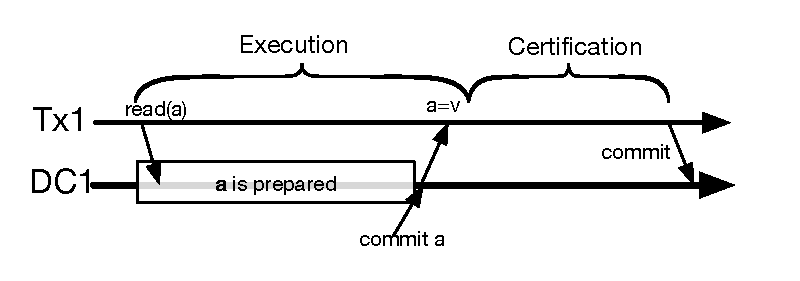
\includegraphics[scale = 0.48]{figures/NoSpeculativeRead}
\caption{\textit{Transaction T2 tries to read prepared value of T1 and gets blocked.} Horizontal lines denote the state of key X and transaction coordinator TC1.}
\label{fig:specula_read}
\vspace{-3mm}
\end{figure}
Speculative commit allows a transaction coordinator to perform optimistic work while its transaction is still being certified, but its transaction's prepared keys are inaccessible for the whole prepare duration. As shown in figure \ref{fig:specula_read}, after speculatively-commit T1, the transaction coordinator, TC1, starts a new transaction T2 that tries to read key X that is prepared by T1. Because key X's final state is unknown, T2 is blocked until T1 finishes. When a system has some frequently accessed data (a.k.a., hotspots), such a blocking scenario may occur frequently. In these scenarios, speculating on transaction commit alone will yield very limited performance benefits.

Speculative read allows transactions to read updates of previous speculatively-committed transactions. More specifically, a transaction is permitted to read transactions finally committed and transactions speculatively-committed at the same node, before it starts (as SPSI property 1 states). A straw-man approach is to allow reading a prepared version if the prepare time is below the reader's snapshot. However, this is problematic for our targeting setting: data is partially replicated, so a speculative transaction's data may be in remote servers; a speculative transaction can be prepared in different partitions with different timestamps, so reading with the same timestamp does not guarantee including all updates of a transaction to read. Therefore, we rely on the aforementioned speculative commit phase to ensure SPSI property 1: it essentially applies a speculatively-committed transaction's updates (even data that is not replicated locally) to local storage with a speculative-commit timestamp. Due to this guarantee, we devised a simple speculative read rule: with a snapshot time, a transaction is permitted to read local speculative records with 'speculative-commit timestamp' smaller than its snapshot time.

Speculative read develops \textit{data dependency}, such that a transaction that has read speculative data can not commit, until the transaction it has read from commits or aborts. A speculative read can have two outcomes: if the speculative transaction finally commits, with a commit timestamp no larger than the commit time of the transaction, the read can commit; on the other hand, if the speculative transaction aborts, or commits with a larger timestamp, the speculative version should not belong to the snapshot of the read so the reader should be aborted.
\fi


\subsection{Reducing transaction's logical duration}
\label{sub:pc}
Speculative read can improves throughput when an optimistic guess is often correct: the pre-commit data versions that a transaction has read will commit with timestamps below the reader's snapshot. Thus, the effect of speculative read highly depends on the underlying timestamp assignment scheme: even if transactions has high commit rate, if they are always assigned large commit timestamps, their readers are still likely to be aborted. Intuitively, an ideal timestamp assignment scheme should assign commit timestamps as small as possible, while not violating SI and SPSI. State-of-the-art decentralized transactional protocols \cite{clocksi, pileus, spanner} typically uses a timestamp assignment scheme as follows: each data partition (or server) employs a scalar clock (either physical, logical or hybrid); the scalar clock increases monotonically, and is updated when the partition receives read or prepare requests (physical clocks advances automatically); a partition proposes its scalar clock as the prepare time for a prepare request; the commit time of a transaction is calculated as the maximal of prepare time from all involved partitions. As each partition has only one scalar clock, the timestamp proposed to a transaction involving that partitions is inevitably affected by all other transactions that have accessed that partition, which results in generally large timestamp. To mitigate this problem, we propose a time assignment scheme, namely \textit{Precise Clock}, that produces small logical duration for transactions. Essentially, we preserve a scalar clock per key and use the scalar clock to track precisely the read/write relation happened to a key, to only propose a timestamp that is necessary to ensure not breaking SI and SPSI. 



\iffalse
\begin{figure}[tbh]
\centering
\hspace{-6mm}
\centering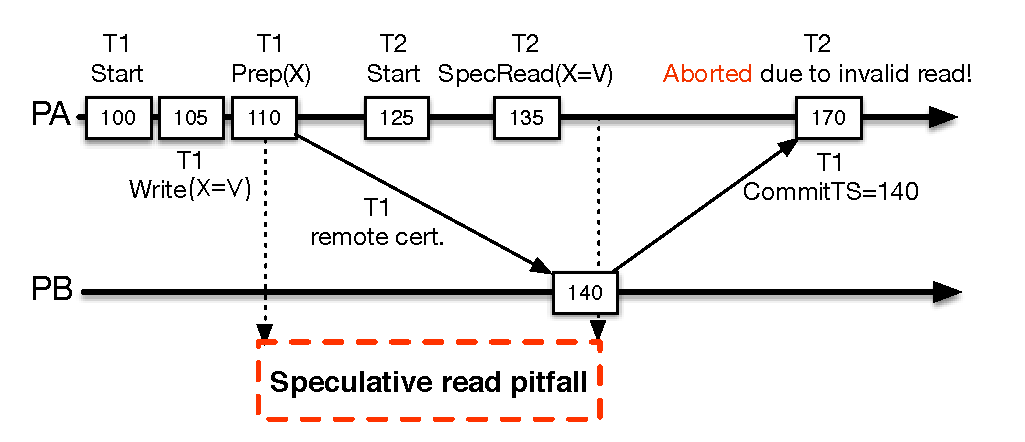
\includegraphics[scale = 0.48]{figures/SpeculativeRead}
\caption{\textit{Transaction reading an invalid prepared version.} Horizontal lines denote two distant partitions PA and PB. Numbers in boxes denote a partition's physical time.}
\label{fig:specula_read}
\end{figure}


\textit{Precise Clock} strikes to propose small prepare timestamps, while not violating any properties of SI or SPSI. On the contrary, we find that the current timestamp assignment scheme proposes unnecessarily large prepare timestamps. Protocols like \cite{clocksi, spanner} enforce each partition to propose monotonically-increasing (physical) timestamps than previous received events (timestamps of read and prepare). In essence, this ensures that after a transaction read a key from a partition, further transactions that update that key can only commit with a larger timestamp than the previous reader's snapshot time, so that the reader's snapshot remains unchanged and thus consistent. However, under this rule, even transactions that update disjoint keys will get higher timestamp than the reader's snapshot time. It is easy to see that this is not necessary: imagine the current protocol is applied to a datastore where each partition only contains a single key; in that case, non-conflicting transactions, which would access the same partition due to data placement, will access disjoint partitions and get different timestamps. Based on this intuition, we propose a new scheme that \textbf{precisely} tracks the read/write causal relations and tries to propose minimal prepare time. We combine the use of physical and logical clocks (as in \ref{hybridclock, bravoclock}): our scheme still uses physical time as a transaction's snapshot time, but maintains a logical clock per key to track the timestamp of transactions that have read the key, i.e. \textit{high time}. We give its read and prepare protocols below. Its pesudo-code will be presented together with the \specula protocol. 
\fi

\iffalse
 and we will discuss its correctness.
\fi

\subsubsection{Pipelining speculative transactions}
As have been discussed in \textbf{cite the right section}, we allow speculatively committing transactions and externalizes speculative results to clients, to further increase throughput and reduce latency. Due to the help of SPSI, the externalized speculative snapshot still provides stringent guarantees \textbf{be more precise here}, which spares developers from having to handle concurrency anomalies as in other well-known weak consistency models \cite{cops, dynamo}. A client can speculatively commit multiple transactions, i.e. pipelining speculative transactions. To capture the potential causal dependency between a client's subsequent transactions, we develop \textbf{flow dependence} for a client's speculative transactions: if a speculative transaction is aborted, the client's following transactions issued after the aborted one will be aborted; moreover, a transaction can not commit before its dependent transactions commit. The maximal number of speculative transactions a client can pipeline impacts performance, but there is no clear-cut answer: higher number of speculative transactions, a.k.a larger speculation depth, can achieve higher throughput when transaction commit rate is high, but it leads to larger number of cascading aborts when commit rate is low. We propose a simple black-box auto-tuning method that we will discuss further and evaluate.

\subsection{Speculative protocol execution}
\label{subsec:execution}

We first give the execution of precise clock.
\begin{itemize}
\item \textbf{Read} When a transaction $T_x$ reads a key K, it is blocked if K is currently being prepared with a prepare time smaller than $T_x$'s snapshot ($ST_x$). Otherwise, $Tx$ reads K's highest version below $ST_x$ and updates K's high time (HT) to $max(HT, ST_x)$.
\item \textbf{Prepare} When preparing K, a transaction $T_y$ gets prepare time as $max(HT, ST_y)+1$. $T_y's$ commit timestamp is the maximal of the prepare time for all keys of its write-set.
\end{itemize}

\paragraph{Start transaction and execution} As in the baseline protocol, a transaction is initialized in a server and assigned the server's physical time as its snapshot time (Alg1, lines 1-3). Then it performs a sequences of read and write operations.

\paragraph{Local certification} After the execution all operations, the transaction undergoes the local certification phase. To enforce SPSI property XX \textbf{to ref the correct property}, the transaction's updated keys are sent to their local replicated partitions (no matter the partition is a master or slave replica) to check write-write conflict with committed and speculatively committed transactions. Keys not replicated locally are sent to a local \textbf{cache} partition, which temporarily stores speculative updates to non-local keys created by previous local speculative transactions (Alg1, lines 12-13). A partition replies \textbf{abort} in case conflicts are detected; otherwise, the partition prepares the transaction and proposes a prepare timestamp according to the precise clock rule: for each key, it retrieves the key's $HighTime$ and proposes $HighTime+1$; then the maximal of proposed time for all keys is returned as the prepare timestamp (Alg2, lines 21-23). Essentially, a transaction passed local certification is ensured that, among all keys replicated locally (and temporarily cached keys), the transaction has no conflict with committed transactions and local speculative transactions. Note that at this point, these prepared records are still not visible to other local transactions, as they may be prepared with different timestamps and allowing them to be visible already could violate consistent snapshot.

\iffalse
the transaction coordinator also certifies all keys belonging to local slave partitions and the cache (which contains all keys of speculatively-committed transactions locally, as will be explained in following text), against locally prepared or speculatively-committed transactions and committed transactions (Alg1, line 13). The local cache only temporarily caches speculative updates for local transactions to read. If a transaction's write-set does not conflict with (i.e. overlaps in duration) existing prepared or speculative-committed transactions in a partition, the partition calculates the prepare time for this transaction and prepares each key, or places them in a waiting queue if these keys are already prepared (Alg2, lines 17-18). The timestamp calculation follows the PreciseClock rule, that takes the maximum of the transaction's snapshot time and the high time of all keys to certify (Alg2, lines 14-16). The partition replies to the prepare request if all keys are prepared and replicates its prepared write-set to its replicas (Alg2, lines 20-21). Note that if a transaction tries to read prepared records, it will be blocked as in the baseline protocol.
\fi

\paragraph{Speculative commit} Upon receiving prepared replies from all updated local partitions (including the cache partition), the coordinator calculates the \textit{specula-commit timestamp} for this transaction as the maximal of proposed prepare timestamps and it sends \textbf{spec\_commit} messages to all involved local partitions (Alg1, lines 15-18). Partitions convert prepared records from \textit{prepared} state to \textit{specula-committed} state, with \textit{specula-commit timestamp} (Alg2, lines 24-27). Only by then, these records can be read by local transactions. Meanwhile, the transaction coordinator sends updates to corresponding remote master partitions for remote certification. The local certification step and this step are indeed a 2PC that makes a transaction's speculative updates atomically visible to local transactions (Alg1, lines 19-20). Note that programmers can choose whether to expose this speculative commit guess to clients. While concealing speculative commit is safe, exposing speculative commit can reduce observed latency and allow clients to issue more transactions, but wrong speculation may need complex compensation.

\paragraph{Speculative read}  A transaction's read request for a key is sent to local partitions, if the key is replicated locally; if the key is not locally replicated, before requesting remote replicas, the transaction first tries to read from the local cache to check if previous local speculative transactions has updated that key (Alg1, lines 5-10). A transaction can read all transactions committed before its snapshot (Alg2, lines 5-6) as well as local transactions speculatively committed before the snapshot (Alg2, lines 9-13). Reading a speculative value creates data dependency between the reader and the owner transaction of the speculative value (Alg2, lines 8-10). Additionally, when a key is being read, its high time is updated according to precise clock rule (Alg2, line 2).

\paragraph{Final commit/abort} A transaction coordinator finally commits a transaction, when (i) it has received prepare replies from all updated partitions and their replicas, (ii) all data dependency is resolved, i.e. it has received \textit{'read valid'} notification for all speculatively-read data, and (iii) flow dependency is resolved, i.e. the client has no pending speculative transaction before this transaction. To finally commit a transaction, the transaction coordinator broadcasts the commit decision to all replicas of updated partitions, atomically sets the transaction updates from 'speculatively-committed' to committed state and notifies all readers of this transaction if their read is still valid (Alg2 lines 29-35). Another important condition not presented in the code is that, a speculative transaction can not commit until none of its speculative records have other preceding speculative records. This is because if there is still preceding speculative transaction, this transaction may commit with a large timestamp that causes write-write conflict with the current transaction and leads to abort.

A speculative transaction is aborted if its certification check fails, its speculative reads are invalid, or any of its preceding transactions from the same  client are aborted. To abort a speculative transaction, its coordinator removes its local speculatively-committed updates, aborts all following transactions from the same and notifies \textit{'read aborted'} to all transactions that have read from it. 

\begin{algorithm}[!ht]
\caption{Coordinator protocol}
\label{alg:coord_protocol1}
{
%\footnotesize
\scriptsize
\begin{tabbing}
xxx\=xxxx\=xxxx\=xxxx\=xxxx\=xxxx\=xxxx\kill
$1$\>\textbf{StartTransaction}(Tx)\\
$2$\>\>Tx.Snapshot$\leftarrow$\textit{current\_time()}\\
$3$\>\>Tx.Coord$\leftarrow$\textit{self()}\\
\\
$4$\>\textbf{ReadDataItem}(Tx, Key)\\
$5$\>\>\textbf{if} \textit{in\_tx\_buffer}(Tx, Key) \textbf{then}\\
$6$\>\>\>\textbf{return} \textit{read\_from\_buffer}(Tx, Key)\\
$7$\>\>\textbf{else if} \textit{is\_key\_replicated}(Key) \textbf{then}\\
$8$\>\>\>\textbf{return} \textit{read\_from\_replica}(Tx, Key)\\
$9$\>\>\textbf{else}\\
$10$\>\>\>\textbf{return} \textit{read\_from\_cache}(Tx, Key)\\
\\
$11$\>\textbf{SpeculativeCommit}(Tx)\\
$12$\>\>\textbf{for} \verb {Updates,  \verb Partition} \textbf{in} Tx.WriteSet \\
$13$\>\>\>\textbf{send} \verb {prepare,  \verb Tx,  \verb Updates} \textbf{to} \textit{local(Partition)} \\
$14$\>\>\textbf{wait until}\\
$15$\>\>\>\textbf{receive all} \verb {prepared, \verb Tx,  \verb PrepTime} \\
$16$\>\>\>\>SCTime $\leftarrow$ \textit{max}(\textbf{all} PrepTime)\\
$17$\>\>\>\>\textbf{send} \verb {spec_commit,  \verb Tx,  \verb SCTime} \\
$18$\>\>\>\>\>\textbf{to} \textit{local(Tx.Partitions)}\\
$19$\>\>\>\>\textbf{send} \verb {prepare,  \verb Tx}  to \textit{Tx.RemotePartitions}\\
$20$\>\>\>\>\textbf{return} \verb {spec_commit,  \verb SCTime} \\
$21$\>\>\>\textbf{receive} \verb {abort, \verb Tx} \\
$22$\>\>\>\>\textbf{Abort}(Tx)\\
\\
$23$\>\textbf{Commit}(Tx)\\
$24$\>\>\textit{atomically commit Tx's spec-committed updates}\\
$25$\>\>\>\textit{and remove Tx's cached updates}\\
$26$\>\>\textbf{foreach} \textit{Tr} \textbf{in}
\textit{Tx.ReadBy} \textbf{do}\\
$27$\>\>\>\textbf{if} Tr.Snapshot $>=$ Tx.CommitTime \textbf{then}\\
$28$\>\>\>\>\textbf{send} \verb {read_valid,  \verb Tx}  \textbf{to} \textit{Tr.Coord}\\
$29$\>\>\>\textbf{else}\\
$30$\>\>\>\>\textbf{send} \verb {read_invalid,  \verb Tx}  \textbf{to} \textit{Tr.Coord}\\
$31$\>\>\textit{notify committed to the client}\\
\\
$32$\>\textbf{Abort}(Tx)\\
$33$\>\>\textit{atomically clean Tx's spec-committed updates}\\
$34$\>\>\>\textit{and remove Tx's cached updates}\\
$35$\>\>\textbf{foreach} Tr \textbf{in}
Tx.ReadBy \textbf{do}\\
$36$\>\>\>\textbf{send} \verb {abort,  \verb Tr}  to Tr.coord\\
$37$\>\>\textbf{foreach} Ts \textbf{in}
Tx.Successors \textbf{do}\\
$38$\>\>\>Abort(Ts)\\
$39$\>\>\textit{notify aborted to the client}\\
\end{tabbing}
}
\end{algorithm}

\begin{algorithm}[!ht]
\caption{Server protocol}
\label{alg:server_protocol}
{
%\footnotesize
\scriptsize
\begin{tabbing}
xxx\=xxxx\=xxxx\=xxxx\=xxxx\=xxxx\=xxxx\kill
$1$\>\textbf{upon} receiving message \verb {read,  \verb Tx,  \verb Key} \\
$2$\>\>HighTime.Key$\leftarrow$ max(HighTime.Key, Tx.Snapshot)\\
$3$\>\>\{Tw, State, Value\}$\leftarrow$\\
$4$\>\>\>\>Store.latest\_before(Key, Tx.Snapshot)\\
$5$\>\>\textbf{if} State = committed\\
$6$\>\>\>\textbf{reply} Value\\
$7$\>\>\textbf{else if} State = prepared\\
$8$\>\>\>Tw.WaitingReaders.add(Tx)\\
$9$\>\> \textbf{else if} State = spec-committed\\
$10$\>\>\>\textbf{if} \textit{local\_read()}\\
$11$\>\>\>\>Tw.ReadBy.add(Tx)\\
$12$\>\>\>\>Tx.ReadFrom.add(Tw)\\
$13$\>\>\>\>\textbf{reply} Value\\
$14$\>\>\>\textbf{else}\\
$15$\>\>\>\>Tw.WaitingReaders.add(Tx)\\
\\
$16$\>\textbf{upon} receiving message \verb {prepare,  \verb Tx} \\
$17$\>\>\textbf{foreach} \{Key, Value\} in Tx.WriteSet \textbf{do}\\
$18$\>\>\>\textbf{if} Key is updated by Ty $\wedge$ Ty.State = prepared\\
$19$\>\>\>\>\textbf{wait until} Ty.State = committed \textbf{or} aborted\\
$20$\>\>\textbf{if} CertificationCheck(Tx) is successful\\
$21$\>\>\>PrepTime$\leftarrow$Tx.Snapshot+1\\
$22$\>\>\>\textbf{foreach} \{Key, Value\} in Tx.WriteSet \textbf{do}\\
$23$\>\>\>\>PrepTime$\leftarrow$max(PrepTime, HighTime.Key+1)\\
$24$\>\>\>Store.Key.insert(Tx, \{prepared, Value, PrepTime\})\\
$25$\>\>\>\textbf{send} \verb {prepare,  \verb Tx,  \verb PrepTime}  to \textit{replicas()} \\
$26$\>\>\>\textbf{reply} \verb {prepared,  \verb Tx,  \verb PrepTime} \\
$27$\>\>\textbf{else}\\
$28$\>\>\>\textbf{reply} \verb {aborted, \verb Tx} \\
\\
$29$\>\textbf{upon} receiving message \verb {spec_commit,  \verb Tx,  \verb SCTime} \\
$30$\>\>\textbf{foreach} \{Key, Value\} in Tx.WriteSet \textbf{do}\\
$31$\>\>\>Store.Key.update(Tx, \{spec-committed, Value,\\
$$\>\>\>\> SCTime\})\\
$32$\>\>\>\textit{unblock waiting preparing transactions}\\
$33$\>\>\>\textit{reply to waiting readers}\\
\\
$34$\>\textbf{upon} receiving message \verb {commit,  \verb Tx,  \verb CTime} \\
$35$\>\>\textit{abort conflicting spec-committed or prepared transactions}\\
$36$\>\>\textbf{foreach} \{Key, Value\} in Tx.WriteSet \textbf{do}\\
$37$\>\>\>Store.Key.update(Tx, \{committed, Value, CTime\})\\
$38$\>\>\>\textit{unblock waiting preparing transactions}\\
$39$\>\>\>\textit{reply to waiting readers}\\
\\
$40$\>\textbf{upon} receiving message \verb {abort,  \verb Tx} \\
$41$\>\>\textbf{foreach} \{Key, Value\} in Tx.WriteSet \textbf{do}\\
$42$\>\>\>Store.Key.remove(Tx)\\
$43$\>\>\>\textit{unblock waiting preparing transactions}\\
$44$\>\>\>\textit{reply to waiting readers}
\\

\end{tabbing}
}
\end{algorithm}
\iffalse
\subsection{Correctness}
\subsubsection{PreciseClock} 
We sketch a brief proof to show that PreciseClock provides Snapshot Isolation.
\begin{itemize}
\item \textbf{No write-write conflict} For any concurrent transaction that conflicts, we allow at most one to commit and abort the others.
\item \textbf{Consistent snapshot} While reading a key, if a transaction encounters a prepare record with a smaller timestamp than its snapshot, it is blocked. The transaction is unblocked until that prepared record is removed. If that prepared record is removed due to abort, the transaction will not read it value; otherwise, if that prepared record is committed, the transaction reads it, if its commit time is no larger than the transaction's snapshot. Therefore, a transaction will never read from aborted transactions or transactions with a commit time larger than their snapshot time. On the other hand, after a transaction finishes reading a key, the key's high time will be at least as large as the transaction's snapshot (Alg2, line 2), so no further transaction can commit a new version of this key with timestamp no larger than its snapshot (Alg2, lines 14-16). Therefore, a transaction will never miss values with commit time no larger than its snapshot.
\iffalse
\item \textbf{Transaction commits with a total-order} we can totally order transactions in the following steps: firstly, we order two transactions with their commit timestamp; if they have an identical commit timestamp, we compare each transaction's largest updated key (which we assume to have a total order). Since two transactions with the same commit timestamp must have disjoint key sets (otherwise, at least one would have been aborted), we can derive total order among any two transactions.
\fi
\end{itemize}

\subsubsection{SPSI} 
Due to space limit, here we sketch a high-level proof that a transaction running in SPSI would never observe a state that contains write-write conflict, which may break application invariants. By contraction, we assume that a transaction may observe a set of transactions that some of them have write-write conflict. First, we identify the types of transactions that can exist in the system, in terms of a node: prepared transactions, local speculatively-committed transactions, remote speculatively-committed transactions and committed transactions. Since for a transaction, it can not read remote speculative transactions and prepared transactions, so we restrict the proof to only a set of speculative transactions and committed transactions. There are three combinations: conflicts among speculative transactions, conflicts among committed transactions and conflict among speculative and committed transactions. Apparently, there can not be any conflict among committed transactions, as our protocol do not allow write-write conflicting concurrent transactions to commit. 

On the other hand, a transaction could only be speculatively-committed if it is certified against local committed transactions and speculatively-committed transactions and has no conflict with them. Therefore, the conflict can only be between speculative transactions and committed transactions that can not be certified during local certification. Indeed, the conflict between these transactions could only be for keys that is not replicated in the node, as local certification can not detect this conflict. Imagine a local transaction T1 updates K1 and K2 and a remote transaction T2 updates K2 and K3. They conflict in K2. T2 should commit and T1, although was speculatively-committed, should abort. However, a transaction first tries to read K1 and then read K3. If it reads K1of T1 and K3 of T3, it would contain conflicting transactions. However, as we ensure FIFO order between nodes, when T1's abort decision should have reached the node of T before T fetches K3, so T is aborted before reading invalid value.

\subsection{Discussions}
\paragraph{Fault tolerance}
We discuss about how we could handle the failure of different components.\\\\
\textbf{Client failure} Except for storing the timestamp of latest observed transactions, our protocol does not store any other metadata in the client side. Therefore, the failure of a client does not affect the execution of transactions or the user experience of any other clients. However, the client may lose session guarantee after restart.\\\\
\textbf{Server failure} The failure of a server also brings down its data partitions and transaction coordinators. In our protocol, the master replica and slave replicas of a data partition are synchronously replicated  \textbf{cite view synchrony}, so as long as the failure of a replica is detected, the protocol could exclude that replica and continue execution. On the other hand, currently the state of a transaction coordinator is not replicated, so the failure of a transaction coordinator will block all prepared transactions managed by it to be in prepare states. To tackle that, one could use well-known techniques to replicate the states of transaction coordinator within a single datacenter to survive failure.\\\\
\textbf{Datacenter failure} \textbf{To be filled.}

\paragraph{Local certification}
Local certification adds nearly neligible delay, but could exclude transactions having local conflict to enter remote certification, which increases the success chance of speculation. In the current protocol, local certification denotes certifying a transaction against committed transactions and speculatively-committed transactions of the local node. Nevertheless, the notion of `local' and `remote' is relative. Since servers in the same datacenter can have relative low latency among each other, one could imagine extending the local certification phase to also certify all transactions belonging to other nodes in the same server. This can be an interesting extension to our protocol.

\subsection{Fault tolerance}
With speculation, a client gets the notification of 'speculatively\_commit' of a transaction before its local prepare records are replicated. If failure happens before local write-set is replicated, the transaction state is lost and the client can not recover his previous speculatively-committed transactions. To cope with this issue, one could log the transaction write-set to disk before replying to clients, or replicate it to a node in the same datacenter.
\fi


\section{Evaluation}
\label{sec:evaluation}
We deployed \specula over nine geo-distributed datacenters of Amazon EC2 and evaluated it using both synthetic workloads and realistic benchmarks, namely TPC-C and RUBiS. We report the performance achievable by \specula when using exclusively internal speculation, i.e., speculative reads, and when enabling also external speculation, in which case speculative commits are immediately externalized to clients. In the following, we call the first variant of \specula as  {\specula}-Internal, and to the second one {\specula}-External. This choice allows us to contrast the performance achievable by \specula when speculation is used in a fully transparent way for the application, with the case in which programmers are willing to incur the risk of exposing mispeculations to clients and to develop compensation logic to cope with these scenarios.

%Recall that the use of external speculation  allows us to evaluate the performance achievable 
%
%, which allow us to generate workloads 
%
%a synthetic workload and two realistic applications, namely TPC-C and RUBiS. The evaluation includes two variations of our STR, one that only performs speculative read ({\specula}-Internal) and one that can perform both speculative read and speculative commit ({\specula}-External), against two transactional protocols. The results show that even without externalizing speculative results, we can achieve about 3.5$\times$ speedup for workloads with high local contention and low remote contention. Nevertheless, allowing speculative commit can further reduce latency by XXX. \textbf{How to write latency reduction? For some workload, our final latency is 300 while the baselin is 21000, so we say by a factor or 70? What about for perceived latency?}

%\subsection{\specula variations and baselines}
%We implemented two variations of \specula, namely {\specula}-Internal and  {\specula}-External. {\specula}-Internal only allows speculative read, which means it does not externalize speculative results (with respect to 'internal') and does not require writing compensation logic; on the other hand, {\specula}-External allows both speculative read and speculative commit, which may externalize speculative results. Both protocols are run with an automatic tuning process. The automatic tuning process collects throughput statistics from all servers every twenty seconds \textbf{should I mention that?}, then it calculates the next speculation level and informs all servers. The tuning starts with the most conservative speculation level, i.e. no speculative read and no speculative commit, then proceeds until it finds a speculation level that gives the maximal throughput. The possible speculation levels, from conservative to aggressive, are: no speculative read (No SR), only speculative read (SR, the maximal level {\specula}-Internal can have), speculative read and speculative commit with length one (SR+SL1), ..., till SR+SL8 (the maximal level {\specula}-External can have).

Unless otherwise specified, both \specula variants use the hill-climbing self-tuning mechanism described in \S~\ref{subsec:tuning}. For the case of {\specula}-Internal, the self-tuning mechanism simply determines whether to use or not speculative reads. With {\specula}-External, conversely, the self-tuning mechanism also determines whether, in addition to using speculative reads, also speculative commits should be used and the maximum length, in the [1,8] range, of the speculation chain length.


We use two baseline protocols. The first one employs ClockSI~\cite{clocksi}, a non-speculative  transactional protocol that, like \specula, provides Snapshot Isolation using a decentralized timestamp-based concurrency control mechanism. As the original ClockSI protocol does not support replication, in order to ensure a fair comparison with \specula, we extended it to use the same primary-backup replication mechanism employed by \specula. We refer to this protocol as to ClockSI-Rep. The second baseline aims to emulate protocols, like PLANET \cite{pang2014planet}, which allows for externalizing  to clients  the results of transactions that pass their local certification phase. Unlike \specula, though, PLANET does not allow speculative reads nor supports pipelining of speculative transactions, i.e., clients cannot activate new transactions before final committing any previously speculatively committed transaction. PLANET was originally layered on top of MDCC~\cite{mdcc}, which only supports full data replication. In order to ensure an apple-to-apple comparison with the remaining protocols considered in our study, we implement this baseline by building it atop ClockSI-Rep and allowing each client to speculatively commit one transaction.

% while not allowing speculative read or pipelining speculative transactions. As in the original paper, PLANET is built on top of the MDCC protocol \cite{kraska2013mdcc} and uses a prediction model to decide whether to speculate. Since it is not possible to do an apple-to-apple comparison, we implemented a simplified version of PLANET, by building it atop ClockSI-Rep and additionally allows each client to speculatively commit one transaction. 

\subsection{Experimental setup}
\label{subsec:setup}
We implemented our baseline protocol and \specula in  Erlang, based on \textit{antidote}, a popular open-source platform for evaluating distributed consistency protocols \cite{antidote}.

The system is deployed across the following nine datacenters of Amazon EC2: Ireland(IE), Seoul(SU), Sydney(SY), Oregon(OR), Singapore(SG), North California(CA), Frankfurt(FR), \\ Tokyo(TY) and North Virginia(VA). Each datacenter consists of three m4.large instances (2 VCPU and 8 GB of memory) and each instance holds the master replica of one partition. All DCs form a consistent hashing ring arranged according to the order of the above list; each partition is replicated across the five datacenters that follow the datacenter hosting the master replica of that partition, e.g., 
 the  partitions whose primary replicas are maintained at the CA datacenter are replicated by the 
 FR, TY, VA, IE and SU data centers. Table~\ref{tab:latency} reports the largest network latencies incurred at the various data centers to contact one of its replicas and any other data center in the cluster.
 
%  We interleave DCs from nearby regions in the consistent hash ring, so to reduce the variance in the replication  latencies incurred by different  data centers.
 
% hat different replication groups will have similar latency to perform replication, as shown in table \ref{tab:latency}.

A workload stressor is located at each node of the system, which spawns one thread per emulated client. Each client issues transactions to a pool of local transaction coordinators and retries a transaction if it gets aborted. We use two metrics to evaluate latency: the \textit{final latency} of a transaction is calculated as the time elapsed since the first activation of a transaction  until its final commit (including possible aborts and retries); the \textit{perceived latency} is defined as the time since the first activation of a transaction until its last speculative commit event, i.e., the one after which it is finally committed. Each reported result is obtained  from the average of at least three runs. We omit reporting standard deviations in the plots to enhance their readability, and since they were always lower than 10\% than the reported mean values.

%duration from its first trial to its commit time, and the user perceived latency (for speculative commit) is measured as the duration from its first trial to its last speculative commit (after which it commits). Last but not least, each experiment is run for three times. We discard the aggregate results of the first twenty seconds and show the average value (deviation is low).

\begin{table*}
\small
\begin{center}
  \begin{tabular}{l |  l | l | l| l | l | l| l| l |l } 
     & IE & SU& SY& OR & SG & CA &  FR & TY & VA  \\ \hline
  \textbf{Max latency (replicas)} & 334(SG) & 267(FR) & 321(FR) & 160(SG)  & 337(IE) & 167(FR) & 321(SY)& 212(IE)  &  226(SY)  \\   \hline
  \textbf{Max latency (all)} &  334(SG) &  267(FR) & 321(FR)  & 163(SY) & 337(IE) & 175(SG) & 324(SG)  & 233(FR)  & 226(SY) \\ \hline
  \end{tabular}
\end{center}
\caption{Largest network latency experienced, on average, by a DC to contact any of its  replicas and any other DC (msec).}
\label{tab:latency}
\end{table*}

\subsection{Synthetic workloads}
We start by considering a synthetic benchmark, which allow us to to evaluate \specula's performance in presence of workloads with precisely identifiable and very heterogeneous characteristics.The synthetic benchmark generates transactions with null ``think time'', i.e., client threads issue a new transaction as soon as the previous one is final committed, for ClockSI-REP and {\specula}-Internal, or speculatively committed, for {\specula}-External and PLANET. As such, this benchmark is representative of non-interactive applications, in which transactions are used to support machine-to-machine interactions. (like, e.g., in high frequency trading applications).

%We 
% represent idealistic non-interactive workloads, where each thread issues a new transaction as soon as the previous one is committed (or speculative committed). In these experiments, we pick four representative contention levels to check the performance of these protocols.

\paragraph{Transaction and data access} A transaction reads 10 keys then updates them. When accessing a data partition, 90\% of the accesses goes to a small set of keys in that data partition, which we call a hotspot, and we adjust the size of the hotspot to control contention rate. Each data partition has two million keys, of which one million are only accessible by locally-initiated transactions and the others are only accessible by remote transactions. This allows adjusting in an independent way  the likelihood of contention among transactions initiated by the same local node (local contention) and among transactions originated at remote nodes (remote contention).

We consider four workload scenarios, which we obtain by varying the size of the hotspot size in the local and remote data partitions: i) low local and remote contention, ii) low local  and high remote contention, iii) high local and low remote contention, and iv) high local and remote contention.% We set the size of the local hotspot size

%In the following, we use a hotspot size of 30000 keys 

% denote 30000 keys for the size of local hotspot size as low local contention and 1000 keys as high local contention; according, 15000 keys for a remote hotspot is named low remote contention and 500 keys for high remote contention. 80\% of a transaction's key access goes to local master partitions, while 20\% goes to slave data partitions replicated locally.

\begin{figure*}
\centering
\def\svgwidth{0.98\columnwidth}
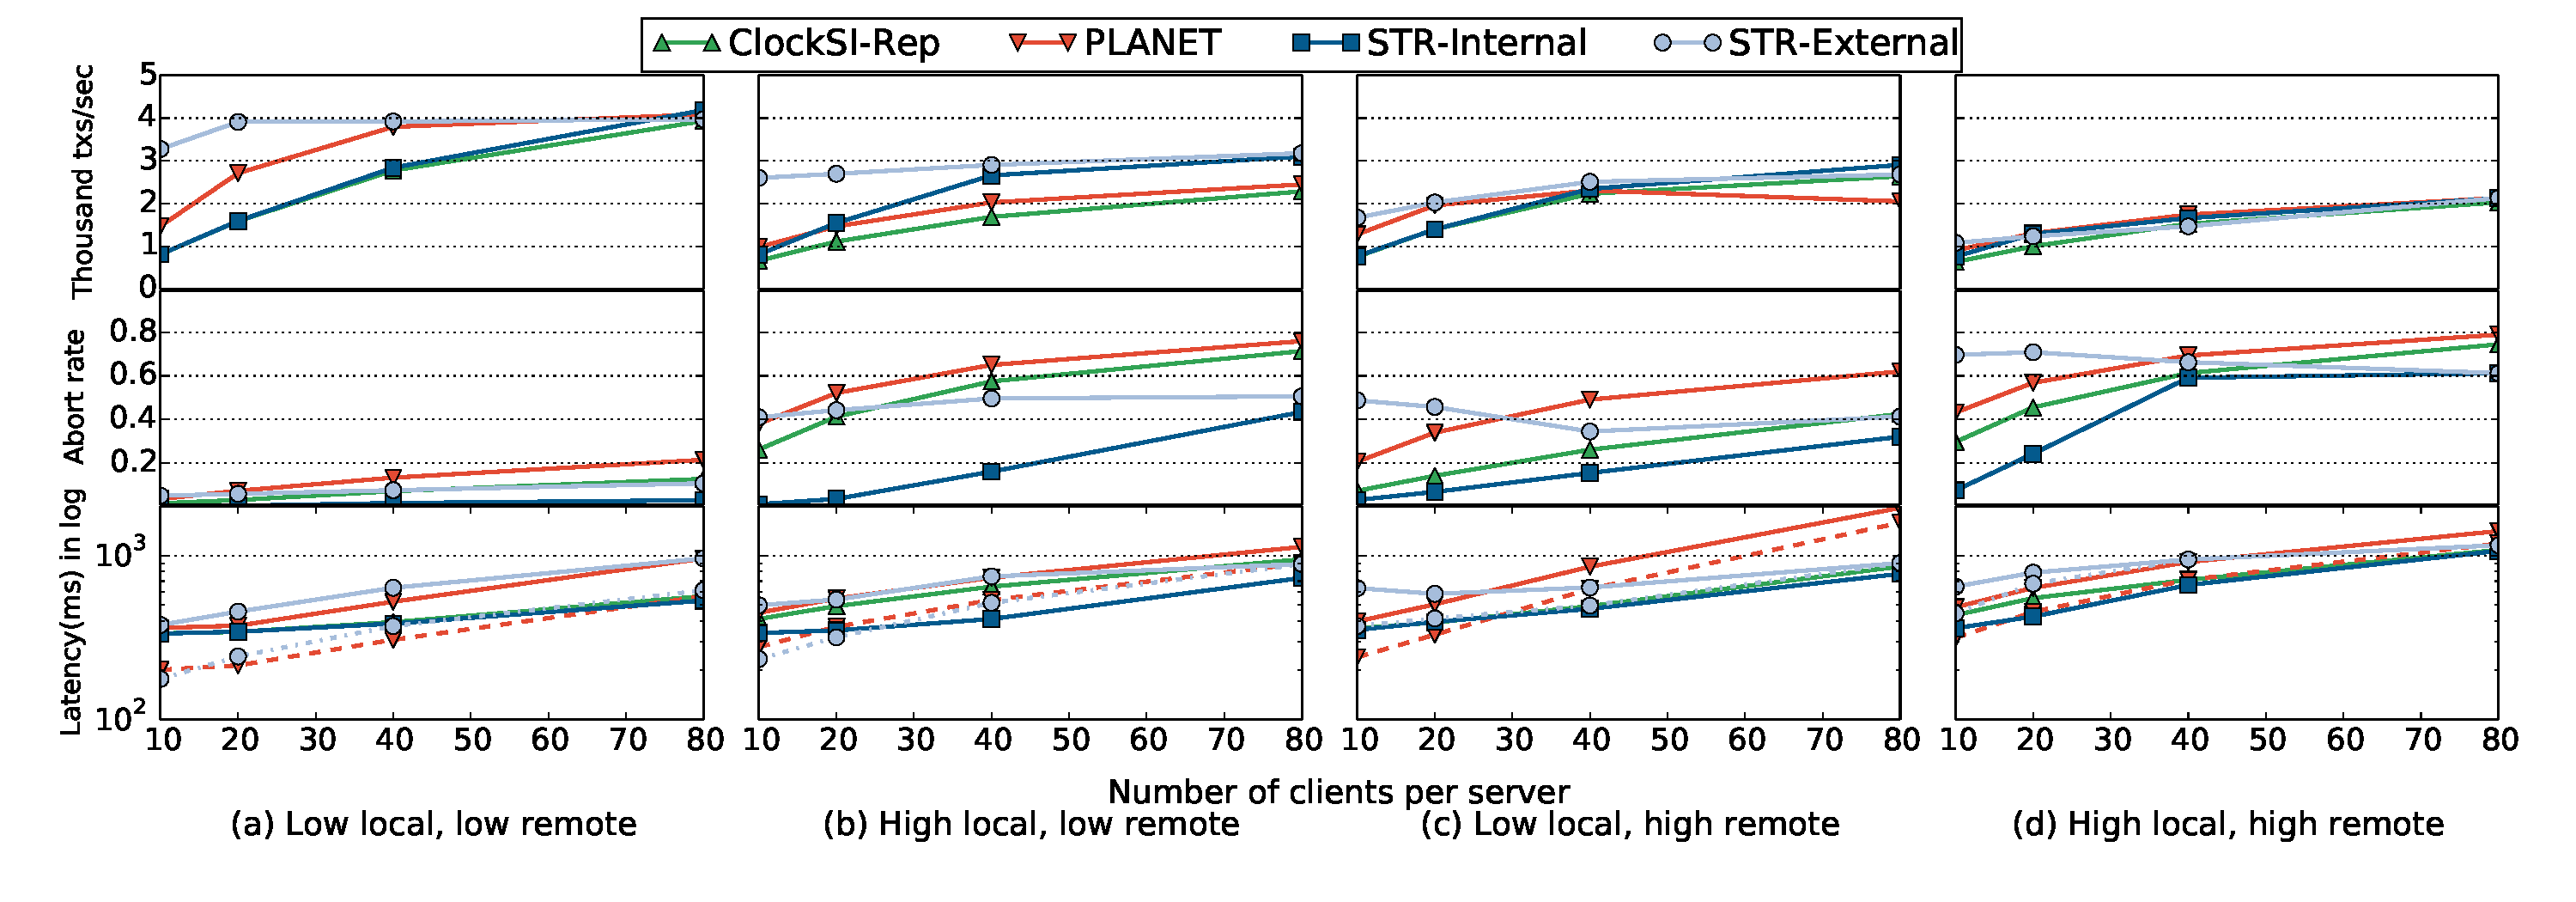
\includegraphics[scale=0.35]{figures/micro}
\vspace{-9mm}
\caption{\small \textit{Performance of different protocols under four levels of contention.} \textit{Low local, high remote} denotes low local contention and high remote contention, and so forth. In the latency plot, we use solid lines for final latency and dashed lines for  perceived latency.}
\label{fig:micro}
\end{figure*}


\begin{figure}[t]
\centering
\def\svgwidth{0.98\columnwidth}
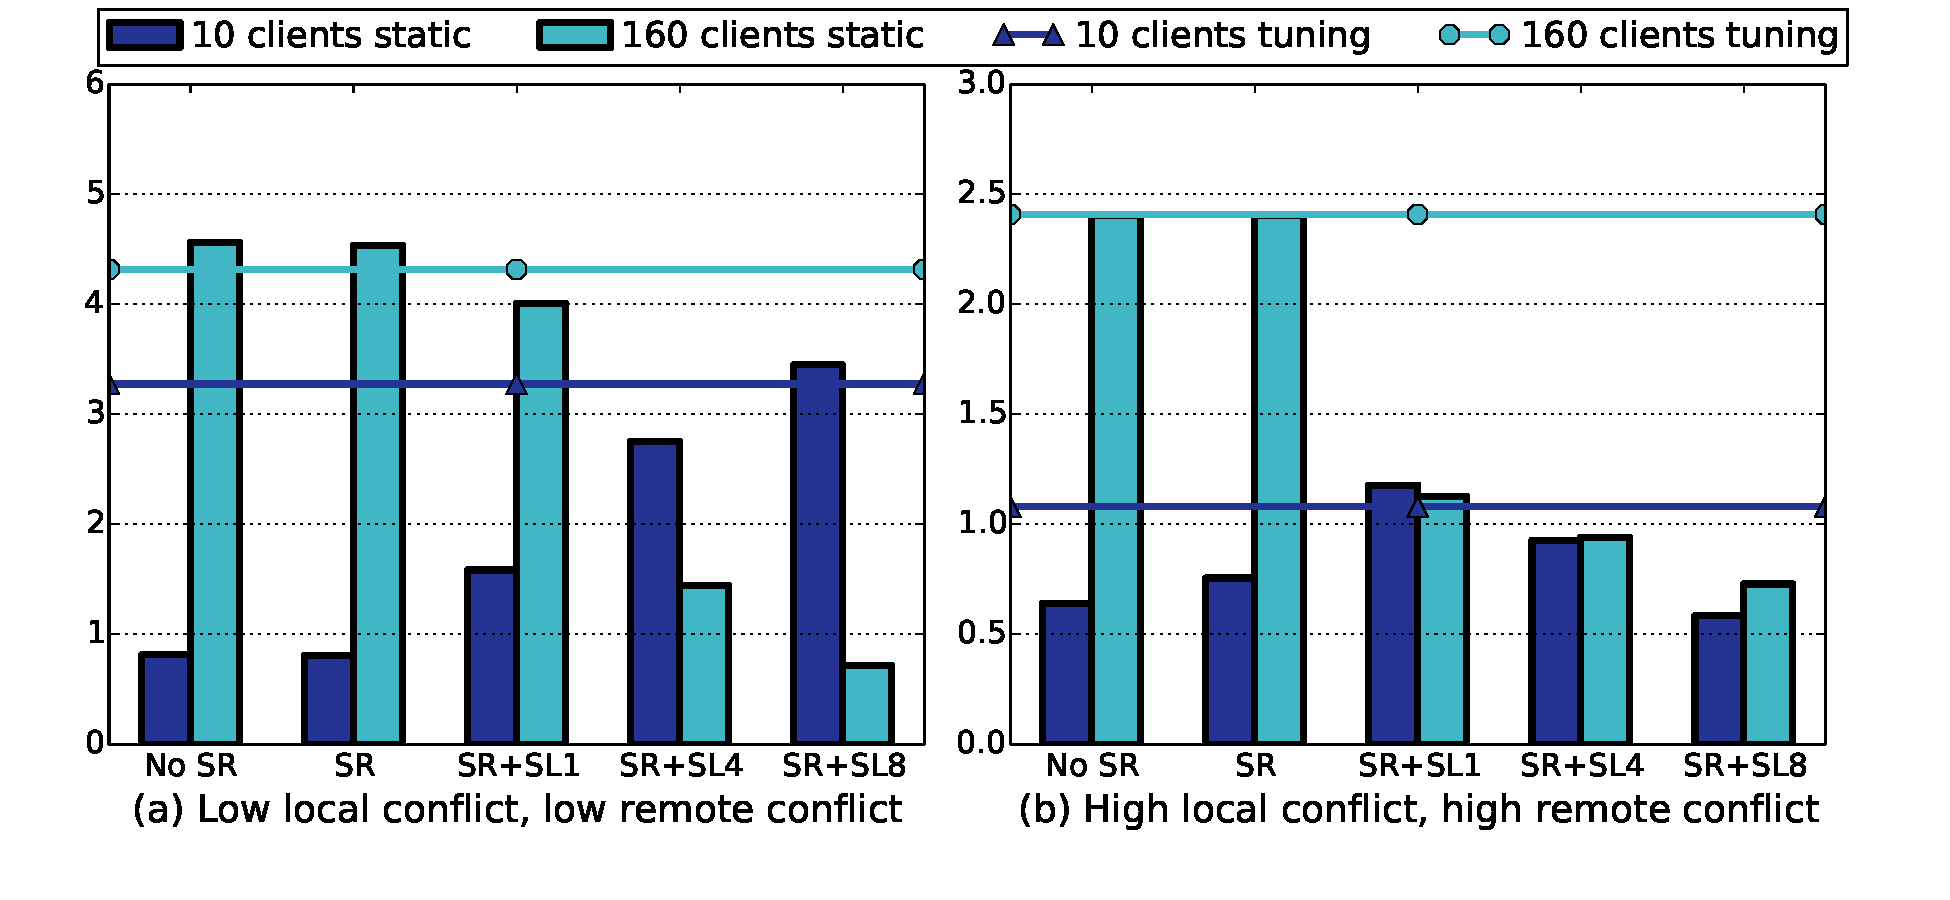
\includegraphics[scale = 0.28]{figures/tuning}
\vspace{-9mm}
\caption{\small The throughput of tuning versus static configuration}
\label{fig:tuning}
\end{figure}

\paragraph{Analysis of the results.} Let us start by considering a workload characterized by both low local contention and low remote contention. As shown in figure \ref{fig:micro}a, both PLANET and {\specula}-External achieve significantly higher throughput than ClockSI-REP when up to 40 clients are used. This can be explained by considering that, with these two protocols, clients can activate one (for the case of PLANET) or more (for the case of  {\specula}-External) new transactions, as soon as they have speculatively committed a transaction. With both ClockSI-REP and  {\specula}-Internal, instead, clients can only initiate a new transaction once they have final committed their previous transactions. In other words, with ClockSI-REP and  {\specula}-Internal, clients submit new transactions at a frequency that is equal to the inverse of the final latency, whereas, with PLANET and   {\specula}-External, the frequency of generation of new transactions is equivalent to the inverse of the perceived latency.

As we can see from the latency plot the perceived latency is about 4$\times$ smaller than the final latency in this workload, in which mispeculation are unlikely to occur given the low contention likelihood. It is worth noting that since {\specula}-External  can support the pipelining of multiple speculative transactions at a given client, this protocol achieves the peak throughput supported by the system (4K txs/sec) with about half of the clients that are required to saturate the system with PLANET (i.e., 20 vs 40 clients). Also, {\specula}-External achieves peak throuhgput gains of  4$\times$ and 2$\times$  when compared with ClockSI-REP and PLANET, respectively.

As the number of clients increases to 80 the use of external speculation in PLANET and {\specula}-External  continues to yield benefits in terms of latency. Yet, this does not reflect directly into a throughput increase vs ClockSI-REP and {\specula}-Internal: with such a large client population, both ClockSI-REP and {\specula}-Internal can fully utilize the available system's resources given that this workload generates very reduced data contention levels.
The  negligible contention generated by this workload creates also little chances of exploiting the speculative read technique, which explain why  {\specula}-Internal and ClockSI-REP achieve almost identical performance. Nonetheless, the use of the PreciseClock mechanisms allows  {\specula}-Internal to achieve a perceivable abort reduction at high load. As with this workload speculative reads are not effective (due to its negligible degree of contention), this experiment allows us to indirectly quantify the overheads introduced by the concurrency control mechanisms used by \specula to support internal speculation (i.e., speculative reads and PreciseClock). Indeed, the fact that the throughputs achieved by ClockSI-REP and  {\specula}-Internal in this workload are  indistinguishable represents an experimental evidence supporting the efficiency of the proposed mechanisms.


Figure \ref{fig:micro}b shows a workload with high local and low remote contention. This is a favourable workload for {\specula}-Internal and {\specula}-External. In fact, these protocols avoid blocking transactions that read pre-committed data records an, this workload, transactions that pass their local certification phase are likely to commit due to the low probability of remote contention. Since PLANET does not use speculative reads, instead, it is forced to frequently block transactions. This leads to an increase of the duration of the transaction execution phase, which makes transactions more vulnerable to conflicts and prone to abort.

As in the previous workload, the throughput gains of  {\specula}-External are particularly large (up to \~4$\times$) with a small number of clients, as this protocol utilizes more effectively than its competitors the available hardware resources thanks to its ability to pipeline successfully the execution of speculatively committed transactions. Unlike in the previous workload, though, both 
\specula variants achieve significant throughput gains also at high client counts, namely approximately 45\% at 40 and 80 clients. This is due to the fact that the use of speculative reads and PreciseClock allow \specula to achieve a higher degree of parallelism among transactions, and hence a higher peak throughput. The ability of \specula to leverage on speculative reads and PreciseClock leads also to a significant reduction of latency and abort rate.

%With 80 clients, both {\specula}-Internal and {\specula}-External achieve about a throughput of about 3K transactions per second, 120\% to the peak throughput of ClockSI-Rep. On the other hand, PLANET achieves little performance gain as transactions often gets blocked during execution and have little chance to speculative commit. The effect of speculative read is directly reflected in latency: when there is low load, the latency of PLANET and ClockSI-Rep considerably increase compared with figure \ref{fig:tuning}a, while the latency of {\specula}-Internal and {\specula}-External are not affected due to speculative read.

Next, we consider two workloads with high remote contention, which are, hence, unfavorable for speculative approaches like \specula. As Figure \ref{fig:micro}c shows, PLANET suffers from large abort rate and  latency, as speculative commit often fails due to high remote contention.
It can be noted that both \specula's variants, instead, achieve much more robust performances than PLANET,  and are at par, or even outperform, ClockSI-REP. As we will discuss more in detail shortly, this is made possible by \specula's self-tuning mechanism, which adapts the degree of aggressiveness of the speculation mechanisms used in the system to the workload characteristics. In this workload, as the number of clients in the sytems grows, along with the likelihood of mispeculations, the self-tuning mechanism opts for progressively disabling both speculative reads and speculative commits, falling back to a conservative/non-speculative processing mode. The last workload, see Figure~\ref{fig:micro}d combines both high local contention and high remote contention, hence further exacerbating the adverseness for speculative techniques. Also, in this case, though \specula's performance remains at par with ClockSI-REP, which does not adopt speculative techniques.  PLANET continues to deliver worst 
latency than the other considered alternatives, although it performs relatively less worse when compared to the previous workload. This is due to the fact that the high likelihood of  local contention causes transactions to detect conflicts in an earlier fashion and to reduce the frequency with which transactions speculative commit (which is harmful in this workload).


\begin{figure*}
\centering
\begin{minipage}{.72\textwidth}
\centering
  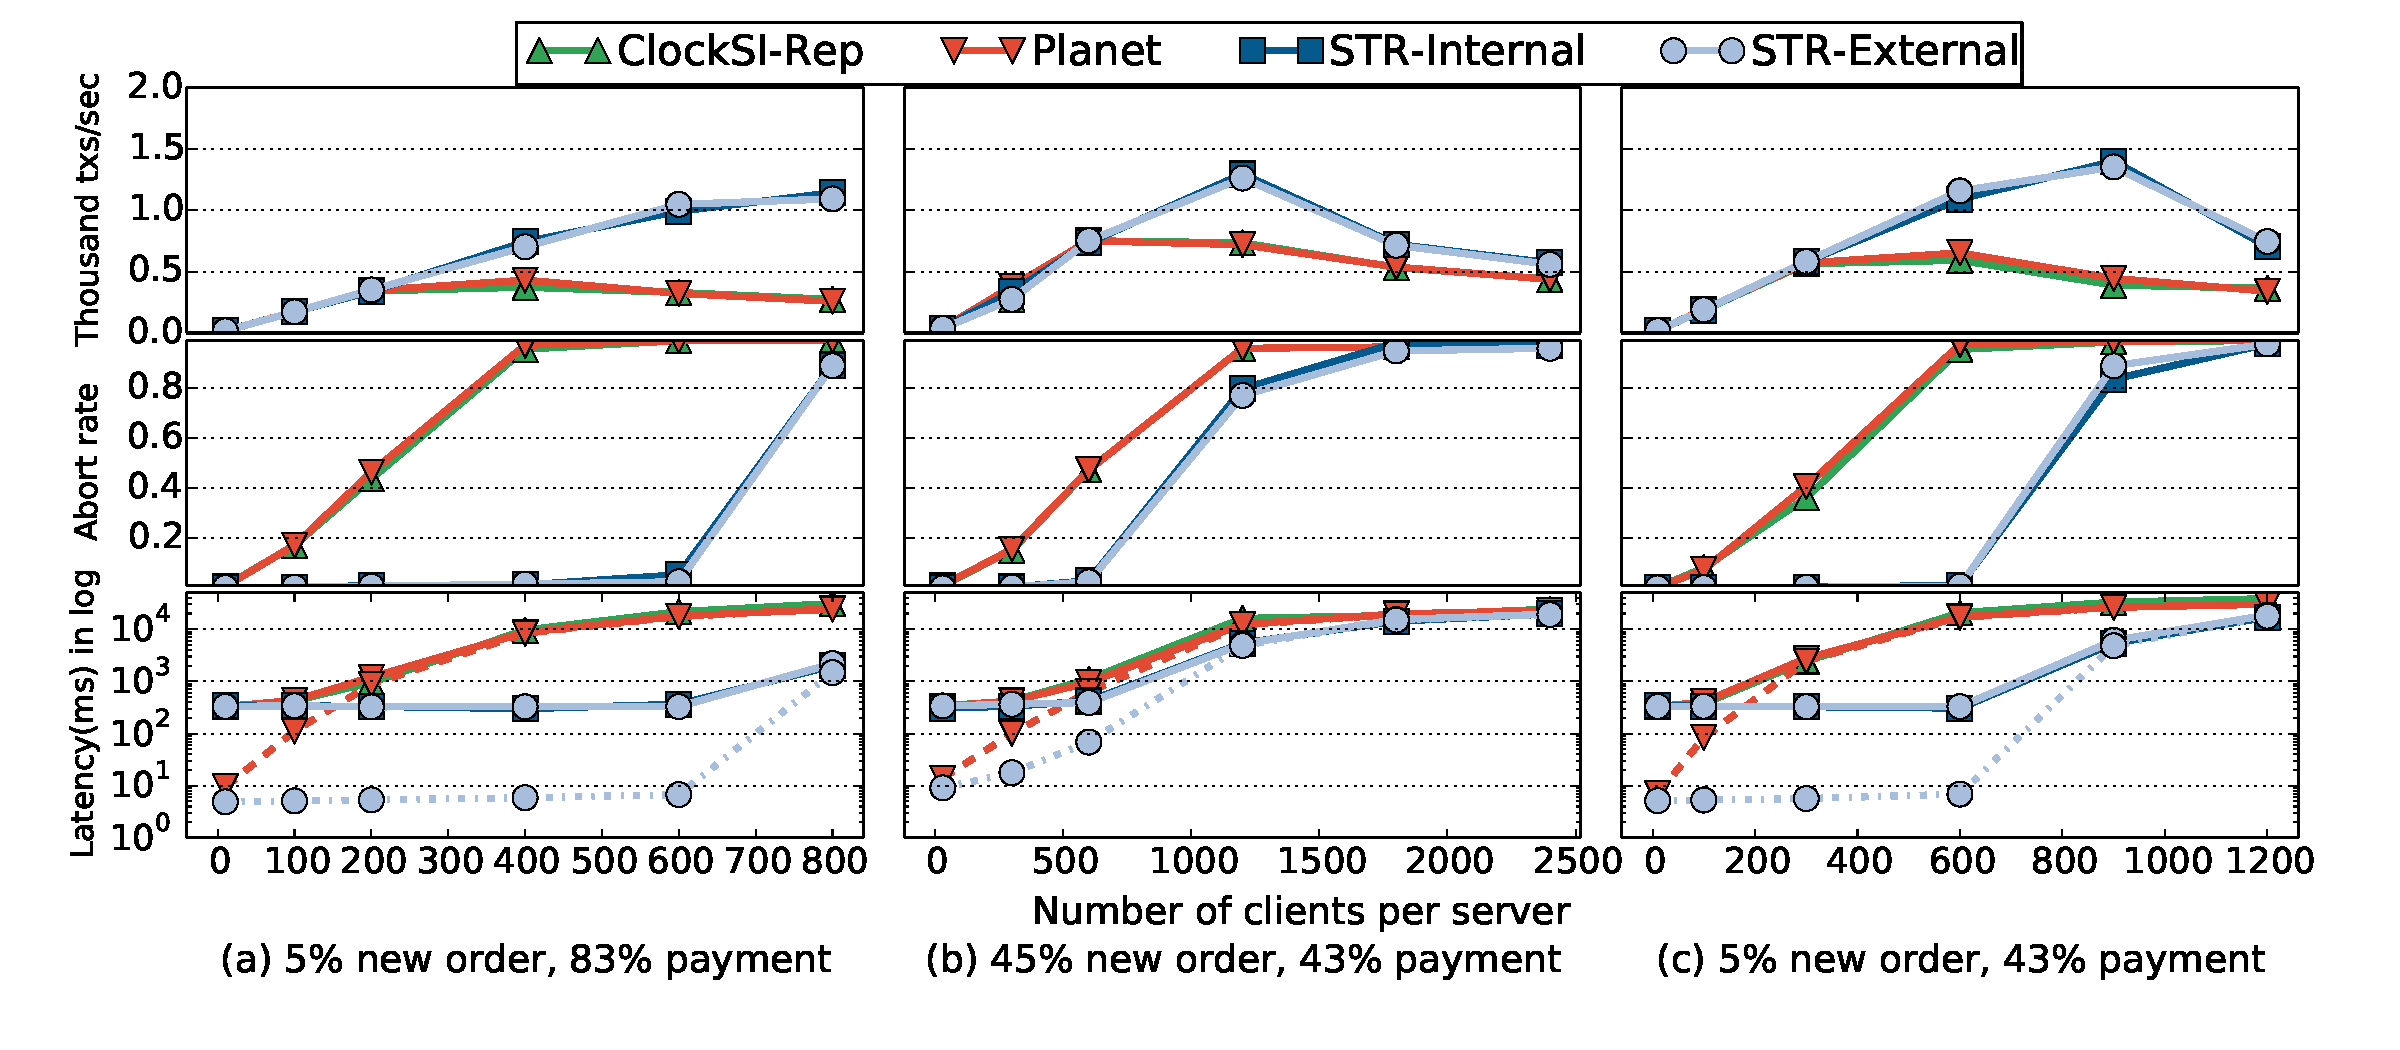
\includegraphics[scale=0.3]{figures/tpcc}
  \vspace{-5mm}
  \caption{\small The performance of different protocols for three TPC-C workloads.}
  \label{fig:tpcc}
\end{minipage}
\begin{minipage}{.26\textwidth}
\centering
  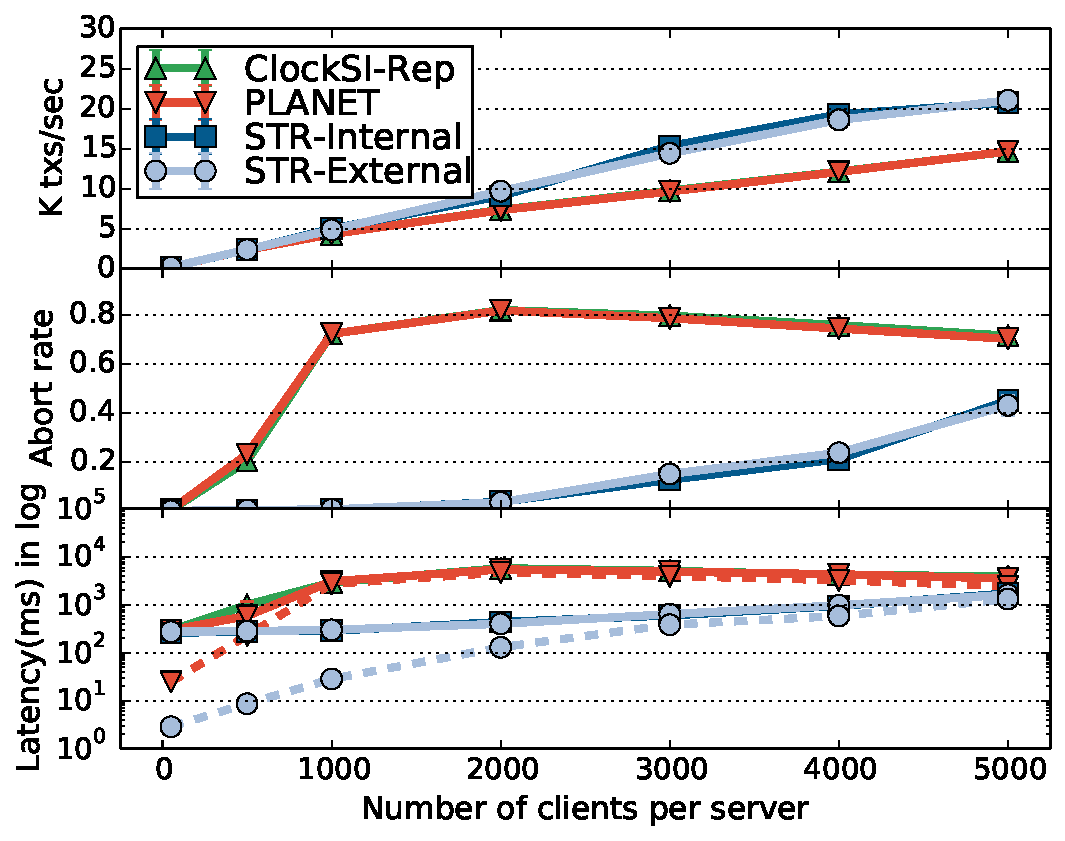
\includegraphics[scale=0.28]{figures/rubislatencywarehouse}
  \vspace{-2mm}
  \caption{\small The performance of different protocols for RUBiS}
  \label{fig:rubis}
\end{minipage}
\end{figure*}


\paragraph{Automatic tuning v.s. static configurations} The previous discussion has shown that \specula's self-tuning mechanism allows for delivering robust performance even in  adverse workload settings. In Figure~\ref{fig:tuning} we report the throughput that \specula would achieve using static configurations of the speculation degree in diverse load and  contention scenarios. The figure shows that the  speculation degree that maximizes throughput varies significantly, and in non-linear ways, as the workload characteristics vary. The data in Figure~\ref{fig:tuning} does not only highlight the relevance of the self-tuning capabilities of \specula. It also provides an experimental evidence of the fact that, once fixed the system's load, the relation between speculation degree and throughput is expressed via convex functions --- a necessary condition to ensure convergence to global optimum for local search strategies such as the one employed by \specula's self-tuning mechanism. This finding supports the design choice of \specula's hill-climbing-based self-tuning strategy, in favour of more complex strategies (like simulated annealing~\cite{hillclimbing}) that sacrifice convergence speed in order to achieve better accuracy in non-convex optimization problems.

% us to design the automatic tuning method. More importantly, as can be seen in the figure, the curve of speculation level to throughput is convex, i.e. if a speculation level gives local maximal throughput, this is guaranteed to be a global maximum throughput. This observation drove the design of the automatic tuning method to be a simple hill climbing algorithm \cite{hillclimbing}: it starts from no speculative read, then proceeds until it finds a local maximal throughput. Despite being simple and fast, this method can reach throughput close to the optimal throughput.



%Reading a key that is not replicated locally causes large latency, which makes it difficult to examine the benefit of speculation. So for most of the experiments, a transaction only accesses keys replicated in local datacenter. We dedicate a separate experiment to examine the effect of remote read on throughput.

\subsection{Macro benchmark}
In the following experiments, we evaluate the performance of \specula with realistic interactive applications, namely TPC-C\cite{tpcc} and RUBiS \cite{rubis}. The key differences between these workloads and the synthetic ones are: (i) while some synthetic workloads already gives severe contention, some transactions of these two applications, e.g. \textit{payment} of TPC-C and \textit{register\_item} of RUBiS, have even more radical contention, which gives \specula better speedup; (ii) to model realistic human to machine interaction, TPC-C and RUBiS specify large ``think time'' between consecutive operations issued by a user, typically a few seconds, which causes speculative commit to not bring obvious performance improvement. Though, speculative commit can still provides low perceived latency.

\subsubsection{TPC-C}
TPC-C \cite{tpcc} models the workload of an online shopping system. We implemented three TPC-C transactions, namely payment, new-order and order-status, according to the specification. Payment transaction has very high local contention and low remote contention; new-order transaction has medium level local and remote contention, and order-status is a read-only transaction. According to the described workload mix rule in the specification, we use three workloads: 5\% new-order, 83\% payment and 12\% order-status (TPC-C A); 5\% new-order, 43\% payment and 52\% order-status (TPC-C B) and 45\% new-order, 43\% payment and 12\% order-status (TPC-C C). We add the ``think time'' and ``key time'' for each transaction as described in the specification, so a client sleeps for some time (from 5 seconds to as large as hundreds of seconds) both before and after issuing a transaction. A server is loaded with five warehouses (more warehouse means less contention), which reaches the server's memory limit.

As we can see in figure \ref{fig:tpcc}, due to having large think time, speculative commit hardly brings any throughput benefit, while speculative read is beneficial due to these workloads all have high local contention. As a result, PLANET achieves the same throughput as ClockSI-Rep, {\specula}-External achieves the same throughput as {\specula}-Internal, and there is a clear throughput difference between STR and the baselines. Though, with low number of clients, PLANET reduces the perceived latency from about 320 millisecond of ClockSI-Rep to about 10 millisecond, by a factor of 32. But when the load increases, the latency of PLANET also increases as local contention is exacerbated. On the other hand, due to allowing speculative read, {\specula}-External and {\specula-Internal} achieve significant speedup compared with the baseline: 2.93$\times$ for TPC-C A, 1.68$\times$ for TPC-C B and 3.47$\times$ for TPC-C C. Both {\specula} protocols also greatly reduce the operation latency by a factor of about 70 compared with the latency of PLANET and ClockSI-Rep.

\subsection{RUBiS}
RUBiS \cite{rubis} models an online bidding system. Of all the 26 user interactions, there are five update transactions: store bid, store buy now, store comment, register item and register user. RUBiS is designed to run on top of a SQL database, so we did the following modification to adapt it to our key-value store: (i) we horizontally partition database tables across servers, so that each server contains an equal portion of data of each table; (ii) many RUBiS insertion operations need to increment a table index to get unique id, which is inefficient when the table is sharded across machines. To avoid this, we let these operations to update local indices that are maintained by local table shards, as studied in \cite{cecchet2008middleware}. We use RUBiS's 15\% update default workload and its default think time (different transactions can have think time from 2 seconds to 10 seconds).

Due to memory limit, we were not able to load the system with more clients. It is hard to saturate servers with TPC-C workloads, because the default workload is dominated by fast read-only transactions and the contention is lower than TPC-C. Nevertheless, the figure \ref{fig:rubis} still shows that \specula achieves good speedup and latency reduction. With 5000 clients, \specula still achieves about 1.43$\times$ speedup compared with ClockSI-Rep and PLANET. Note that the abort rate of PLANET and ClockSI-Rep slightly decreases with increasing number of clients. This is because in RUBiS, the access pattern of a client highly depends on the update of other clients, so with more number of clients, the access pattern gets more diverse and the abort rate is reduced.



\section{Conclusion}
This paper proposed {\specula}, a novel protocol that uses speculative techniques to improve performance of distributed transactions. The three novel speculative techniques, i.e. speculative commit, speculative read and precise clock, collectively mitigate the performance bottleneck of existing transactional protocol. Extensive benchmark showed that our protocol achieves significantly higher throughput than state of the art non-speculative system and is particularly beneficial when workloads have high local conflict and low remote conflict.


% We recommend abbrvnat bibliography style.
\bibliographystyle{abbrv}
\bibliography{references}
\end{document}
